\documentclass[
  % -- opções da classe memoir --
  12pt,				% tamanho da fonte
  %openright,			% capítulos começam em pág ímpar (insere página vazia caso preciso)
  %twoside,			% para impressão em verso e anverso. Oposto a oneside
  oneside,			% para impressão em verso e anverso. Oposto a oneside
  a4paper,			% tamanho do papel.
  % -- opções da classe abntex2 --
  %chapter=TITLE,		% títulos de capítulos convertidos em letras maiúsculas
  %section=TITLE,		% títulos de seções convertidos em letras maiúsculas
  %subsection=TITLE,	% títulos de subseções convertidos em letras maiúsculas
  %subsubsection=TITLE,% títulos de subsubseções convertidos em letras maiúsculas
  % -- opções do pacote babel --
  english,			% idioma adicional para hifenização
  brazil,				% o último idioma é o principal do documento
  % -- opções da classe ime-abntex2 --
  %brasao,
]{ime-abntex2}


% ---
% PACOTES
% ---

\usepackage[utf8]{inputenc}		% Codificacao do documento (conversão automática dos acentos)
\usepackage{float}                    % For improved placement of figures
\usepackage{placeins}                 % Keeps floats 'in their place' with \FloatBarrier
\usepackage{cmap}                     % Mapear caracteres especiais no PDF
\usepackage{lmodern}                  % Usa a fonte Latin Modern
\usepackage{amsmath}                  % Para usar blocos como "gather" de escrever matemática
%\usepackage{amsfonts}                 % Para usar fontes ams
%\usepackage{times}                    % Usa a fonte Times
\usepackage[T1]{fontenc}              % Selecao de codigos de fonte.
%\usepackage{lastpage}                 % Usado pela Ficha catalográfica
\usepackage{indentfirst}              % Indenta o primeiro parágrafo de cada seção.
\usepackage{color}                    % Controle das cores
\usepackage[table]{xcolor}            % Controle das cores em uma tabela
\usepackage{graphicx}                 % Inclusão de gráficos
\usepackage[portuguese]{algorithm2e}  % Para escrever algorítimos
\usepackage{lscape}                   % Para usar landscape
\usepackage{amsthm}                   % Para usar Definições e lemas
\usepackage{amssymb}                  % \mathbb{•}
\usepackage{caption}                  % dependencia de subcaption
%\usepackage{subcaption}               % Para usar \begin{subfigure} e colocar figuras (a) e (b) lado a lado
\usepackage{listings}                 % Para usar \lstinputlisting e incluir código
\usepackage[chapter]{minted}          % Para incluir código com highlight do pygments
\usepackage{breqn}                    % Para quebrar equações grandes em duas linhas
\newtheorem{teo}{Teorema}[section]    % Renomear o comando
\newtheorem{defi}[teo]{Definição}
% o seguinte é necessário para corrigir um bug no algorithm2e
% http://tex.stackexchange.com/questions/113325/problem-with-algorithm2e-and-portuguese-option
\SetKwFor{Para}{para}{fa\c{c}a}{fimpara}
\SetKwBlock{Inicio}{início}{fim}
% não era pra precisar do seguinte, mas precisa para traduzir a captions dos algoritmos
\renewcommand{\algorithmcfname}{Algoritmo}%
% ---

% ---
% Pacotes de citacoes
% ---
% O seguinte serve para mostrar as referencias reversas na bibliografia
% \usepackage[brazilian,hyperpageref]{backref}	 % Paginas com as citações na bibl
\usepackage[alf]{abntex2cite}	% Citações padrão ABNT

% ---
% CONFIGURAÇÕES DE PACOTES
% ---

% ----
% Configuração LISTING
% ----
\def\lstlistingname{Arquivo}
\lstset{                      % general command to set parameter(s)
  %basicstyle=\footnotesize,   % print whole listing small. Possible values:
  %                            %   \footnotesize, \small, \itshape, \ttfamily
  identifierstyle=,           % nothing happens
  commentstyle=\color{white}, % white comments
  stringstyle=\ttfamily,      % typewriter type for strings
  showstringspaces=false      % no special string spaces
}

%\lstset{
%  breaklines=true,
%  breakatwhitespace=false,
%  xleftmargin=1em,
%  frame=single,
%  numbers=left,
%  numbersep=5pt,
%}

\newcommand{\includecode}[2][cpp]{%
  \par Arquivo #2%
  \inputminted[frame=single]{#1}{#2}%
}

% ---
% Configurações do pacote backref
% Usado sem a opção hyperpageref de backref
%\renewcommand{\backrefpagesname}{Citado na(s) página(s):~}
% Texto padrão antes do número das páginas
%\renewcommand{\backref}{}
% Define os textos da citação
%\renewcommand*{\backrefalt}[4]{
%	\ifcase #1 %
%		Nenhuma citação no texto.%
%	\or
%		Citado na página #2.%
%	\else
%		Citado #1 vezes nas páginas #2.%
%	\fi}%
% ---

% as imagens ficam nesse diretório
\graphicspath{{img/}}


% ---
% Informações de dados para CAPA e FOLHA DE ROSTO
% ---
\titulo{Uma Ferramenta de Representação Comportamental Baseado em Otimização
para Futebol de Robôs
%Técnicas de IA Aplicadas a Sistemas Multiagentes Cooperativos e Competitivos
}
\autor{Jan Segre\\Victor Bramigk}
\local{Rio de Janeiro}
\data{Maio de 2015}
\orientador{Paulo Fernando Ferreira Rosa}{Ph.D., do IME}
\coorientador{Bruno Eduardo Madeira}%{M.Sc., do IME}
\instituicao{%
  Instituto Militar de Engenharia
  \par
  Seção de Computação
  \par
  Graduação em Engenharia de Computação
}
\tipotrabalho{Iniciação à Pesquisa}
% O preambulo deve conter o tipo do trabalho, o objetivo,
% o nome da instituição e a área de concentração
\preambulo{Projeto Final de Curso de Graduação em Engenharia de Computação do
Instituto Militar de Engenharia.}
% ---


% ---
% Configurações de aparência do PDF final

% alterando o aspecto da cor azul
%\definecolor{blue}{RGB}{41,5,195}
\definecolor{blue}{RGB}{0,0,0}

% informações do PDF
\makeatletter
\hypersetup{%
  %pagebackref=true,
  pdftitle={\@title},
  pdfauthor={\@author},
  pdfsubject={\imprimirpreambulo},
  pdfcreator={LaTeX with abnTeX2},
  pdfkeywords={ime}{robocup}{analise}{logs}{rede neural},
  colorlinks=true,		% false: boxed links; true: colored links
  linkcolor=blue,			% color of internal links
  citecolor=blue,			% color of links to bibliography
  filecolor=magenta,		% color of file links
  urlcolor=blue,
  bookmarksdepth=4
}
\makeatother
% ---

% ---
% Espaçamentos entre linhas e parágrafos
% ---

% O tamanho do parágrafo é dado por:
%\setlength{\parindent}{1.3cm}

% Controle do espaçamento entre um parágrafo e outro:
%\setlength{\parskip}{0.2cm}  % tente também \onelineskip
\setlength{\parskip}{\onelineskip}

% ---
% compila o indice
% ---
\makeindex
% ---

% ----
% Início do documento
% ----
\begin{document}

% Retira espaço extra obsoleto entre as frases.
%\frenchspacing

% ----------------------------------------------------------
% ELEMENTOS PRÉ-TEXTUAIS
% ----------------------------------------------------------
% \pretextual

% ---
% Capa
% ---
\imprimircapa
%\input{pre_textuais/capa}
% ---

% ---
% Folha de rosto
% (o * indica que haverá a ficha bibliográfica)
% ---
\imprimirfolhaderosto*
%\input{pre_textuais/folha_de_rosto}
% ---

% ---
% Inserir a ficha bibliografica
% ---

% Isto é um exemplo de Ficha Catalográfica, ou ``Dados internacionais de
% catalogação-na-publicação''. Você pode utilizar este modelo como referência.
% Porém, provavelmente a biblioteca da sua universidade lhe fornecerá um PDF
% com a ficha catalográfica definitiva após a defesa do trabalho. Quando estiver
% com o documento, salve-o como PDF no diretório do seu projeto e substitua todo
% o conteúdo de implementação deste arquivo pelo comando abaixo:
%
% \begin{fichacatalografica}
%     \includepdf{fig_ficha_catalografica.pdf}
% \end{fichacatalografica}
\imprimirfichacatalografica
{629.892}
{S455h}
{Segre, Jan}
{Projeto de Fim de Curso (PFC)}
{%
  1. Curso de engenharia da computação - Projeto Final de Curso.
  2. Robótica.
%  3. Minimax.
  3. Otimização.
  I. Bramigk, Victor.
  II. Rosa, Paulo Fernando Ferreira.
  III. Bruno Eduardo Madeira.
  IV. \@title.
  V. Instituto Militar de Engenharia.
}
{Uma ferramenta de representação comportamental baseado em otimizacao
para futebol de robôs}
%{Técnicas de IA aplicadas a sistemas multiagentes cooperativos e
%competitivos}
% ---

% ---
% Inserir errata
% ---
%\begin{errata}
%Elemento opcional da \citeonline[4.2.1.2]{NBR14724:2011}. Exemplo:
%
%\vspace{\onelineskip}
%
%FERRIGNO, C. R. A. \textbf{Tratamento de neoplasias ósseas apendiculares com
%reimplantação de enxerto ósseo autólogo autoclavado associado ao plasma
%rico em plaquetas}: estudo crítico na cirurgia de preservação de membro em
%cães. 2011. 128 f. Tese (Livre-Docência) - Faculdade de Medicina Veterinária e
%Zootecnia, Universidade de São Paulo, São Paulo, 2011.
%
%\begin{table}[htb]
%\center
%\footnotesize
%\begin{tabular}{|p{1.4cm}|p{1cm}|p{3cm}|p{3cm}|}
%  \hline
%   \textbf{Folha} & \textbf{Linha}  & \textbf{Onde se lê}  & \textbf{Leia-se}  \\
%    \hline
%    1 & 10 & auto-conclavo & autoconclavo\\
%   \hline
%\end{tabular}
%\end{table}
%
%\end{errata}
% ---

% ---
% Inserir folha de aprovação
% ---
%
% Isto é um exemplo de Folha de aprovação, elemento obrigatório da NBR
% 14724/2011 (seção 4.2.1.3). Você pode utilizar este modelo até a aprovação
% do trabalho. Após isso, substitua todo o conteúdo deste arquivo por uma
% imagem da página assinada pela banca com o comando abaixo:
%
% \includepdf{folhadeaprovacao_final.pdf}
%
\convidadoum{Bruno Eduardo Madeira}{M.Sc., do IME}
\convidadodois{Julio Cesar Duarte}{D.Sc., do IME}
\imprimirfolhadeaprovacao{25 de maio de 2015}
% ---

% ---
% Dedicatória
% ---
%\begin{dedicatoria}
%   \vspace*{\fill}
%   \centering
%   \noindent
%   \textit{ Este trabalho é dedicado às crianças adultas que,\\
%   quando pequenas, sonharam em se tornar cientistas.} \vspace*{\fill}
%\end{dedicatoria}
% ---

% ---
% Agradecimentos
% ---
%\begin{agradecimentos}
%Os agradecimentos principais são direcionados à Gerald Weber, Miguel Frasson,
%Leslie H. Watter, Bruno Parente Lima, Flávio de Vasconcellos Corrêa, Otavio Real
%Salvador, Renato Machnievscz\footnote{Os nomes dos integrantes do primeiro
%projeto abn\TeX\ foram extraídos de
%\url{http://codigolivre.org.br/projects/abntex/}} e todos aqueles que
%contribuíram para que a produção de trabalhos acadêmicos conforme
%as normas ABNT com \LaTeX\ fosse possível.
%
%Agradecimentos especiais são direcionados ao Centro de Pesquisa em Arquitetura
%da Informação\footnote{\url{http://www.cpai.unb.br/}} da Universidade de
%Brasília (CPAI), ao grupo de usuários
%\emph{latex-br}\footnote{\url{http://groups.google.com/group/latex-br}} e aos
%novos voluntários do grupo
%\emph{\abnTeX}\footnote{\url{http://groups.google.com/group/abntex2} e
%\url{http://abntex2.googlecode.com/}}~que contribuíram e que ainda
%contribuirão para a evolução do \abnTeX.
%
%\end{agradecimentos}
% ---

% ---
% Epígrafe
% ---
%\begin{epigrafe}
%    \vspace*{\fill}
%	\begin{flushright}
%		\textit{``Não vos amoldeis às estruturas deste mundo, \\
%		mas transformai-vos pela renovação da mente, \\
%		a fim de distinguir qual é a vontade de Deus: \\
%		o que é bom, o que Lhe é agradável, o que é perfeito.\\
%		(Bíblia Sagrada, Romanos 12, 2)}
%	\end{flushright}
%\end{epigrafe}
% ---

% ---
% RESUMOS
% ---
% resumo em português
\setlength{\absparsep}{18pt} % ajusta o espaçamento dos parágrafos do resumo
\begin{resumo}

  Este trabalho apresenta uma ferramenta de representação comportamental baseada
  em otimização para futebol de robôs para uma equipe da \textit{Small Size
  League} (SSL) da RoboCup, RoboIME (representando IME nesta competição).
  Equipes da SSL são geralmente controlados por heurísticas puras. Isso
  restringe o movimento dos robôs para um conjunto fixo de comportamentos,
  limitando as possíveis jogadas.

  O objetivo deste trabalho é desenvolver uma ferramenta de representação
  comportamental baseada em otimização para futebol de robôs.

  Um modelo discreto e sequencial no domínio das ações foi criado, juntamente
  com uma função utilidade. Isso possibilitou que uma busca seja feita para
  encontrar jogadas com boa avaliação de acordo com essa função. Foi
  implementada uma arquitetura de controle baseada nessa abstração, onde é feita
  uma busca pela combinação do método de descida do gradiente aplicado a um
  conjunto de jogadas aleatórios, ações sugeridas (inseridos através da GUI) e o
  planejamento anterior. A ferramenta é capaz de controlar um conjunto de robôs,
  dando origem a comportamentos que vão desde bloquear chutes diretos, avançar
  para a quadra adversária e se posicionar para atacar através de passes.

  \textbf{Palavras-chaves}: inteligência artificial, discretização, otimização, robótica, robocup.
\end{resumo}

% resumo em inglês
\begin{resumo}[Abstract]\begin{otherlanguage*}{english}

  This paper presents a behavioral representation tool based on optimization for
  robot soccer for a RoboCup's Small Size League (SSL) team, RoboIME
  (representing IME in this competition). SSL teams are usually controlled by
  pure heuristics. This restricts the movement of the robots to a fixed set of
  behaviors, limiting the possible plays.

  The objective of this work is to develop a behavioral representation tool
  based on optimization for robot soccer.

  A discreet and sequential model in the field of actions was created, along
  with a utility function. This enabled a search to be made to find plays with
  good evaluation according to that function. A control architecture based on
  this abstraction was implemented, where a search is made by combining a
  gradient descent method applied to a set of random moves, suggested actions
  (inserted through the GUI) and the previous planning. The tool is able to
  control a set of robot, yielding behaviors which range from blocking direct
  kicks, advancing to the opponent's court and positioning for attacking through
  passes.

  \textbf{Keywords}: artificial intelligence, discretization, optimization, robotics, robocup.
\end{otherlanguage*}\end{resumo}

% vim: tw=80 et ts=2 sw=2 sts=2 ft=tex spelllang=pt_br,en


% ---
% inserir o sumario
% ---
\pdfbookmark[0]{\contentsname}{toc}
\tableofcontents*
\cleardoublepage
% ---

% ---
% inserir lista de ilustrações
% ---
\pdfbookmark[0]{\listfigurename}{lof}
\listoffigures*
\cleardoublepage
% ---

% ---
% inserir lista de tabelas
% ---
%\pdfbookmark[0]{\listtablename}{lot}
%\listoftables*
%\cleardoublepage
% ---

% ---
% inserir lista de abreviaturas e siglas
% ---
\begin{siglas}
  \item[API] \textit{Application Programming Interface}
  \item[IA] Inteligência Artificial
  \item[SSL] \textit{Small Size League}
  \item[Robocup] \textit{Robotics World Cup}
  \item[RoboIME] Equipe de alunos do Laboratório de Robótica do IME
\end{siglas}
% ---

% ---
% inserir lista de símbolos
% ---
%\begin{simbolos}
%  \item[$ \Gamma $] Letra grega Gama
%  \item[$ \Lambda $] Lambda
%  \item[$ \zeta $] Letra grega minúscula zeta
%  \item[$ \in $] Pertence
%\end{simbolos}
% ---



% ----------------------------------------------------------
% ELEMENTOS TEXTUAIS
% ----------------------------------------------------------
\textual

% ----------------------------------------------------------
% Introdução
% ----------------------------------------------------------
\chapter{Introdução}

A robótica é um ramo da tecnologia que lida com a concepção, construção,
operação e aplicação de máquinas capazes de realizar uma série de ações de
maneira autônoma.  Atualmente é um tópico em rápida ascensão.  Pesquisar,
projetar e fábricar novos robôs serve vários propósitos práticos tais como
domésticos, comerciais e militares.  Um dos problemas atuas da robótica é o
planejamento em ambientes multiagentes dinâmicos e competitivos.  Um exemplo de
um problema dessa classe é um jogo de futebol de robôs, onde um grupo de robôs é
controlado por uma IA independente.
A Figura~\ref{fig:robocup2013} mostra uma imagem da Robocup 2013, competição
internacional de robótica, onde a equipe RoboIME (de alunos do Laboratório de
Robótica do IME) participou.

\begin{figure}[h]
  \centering
  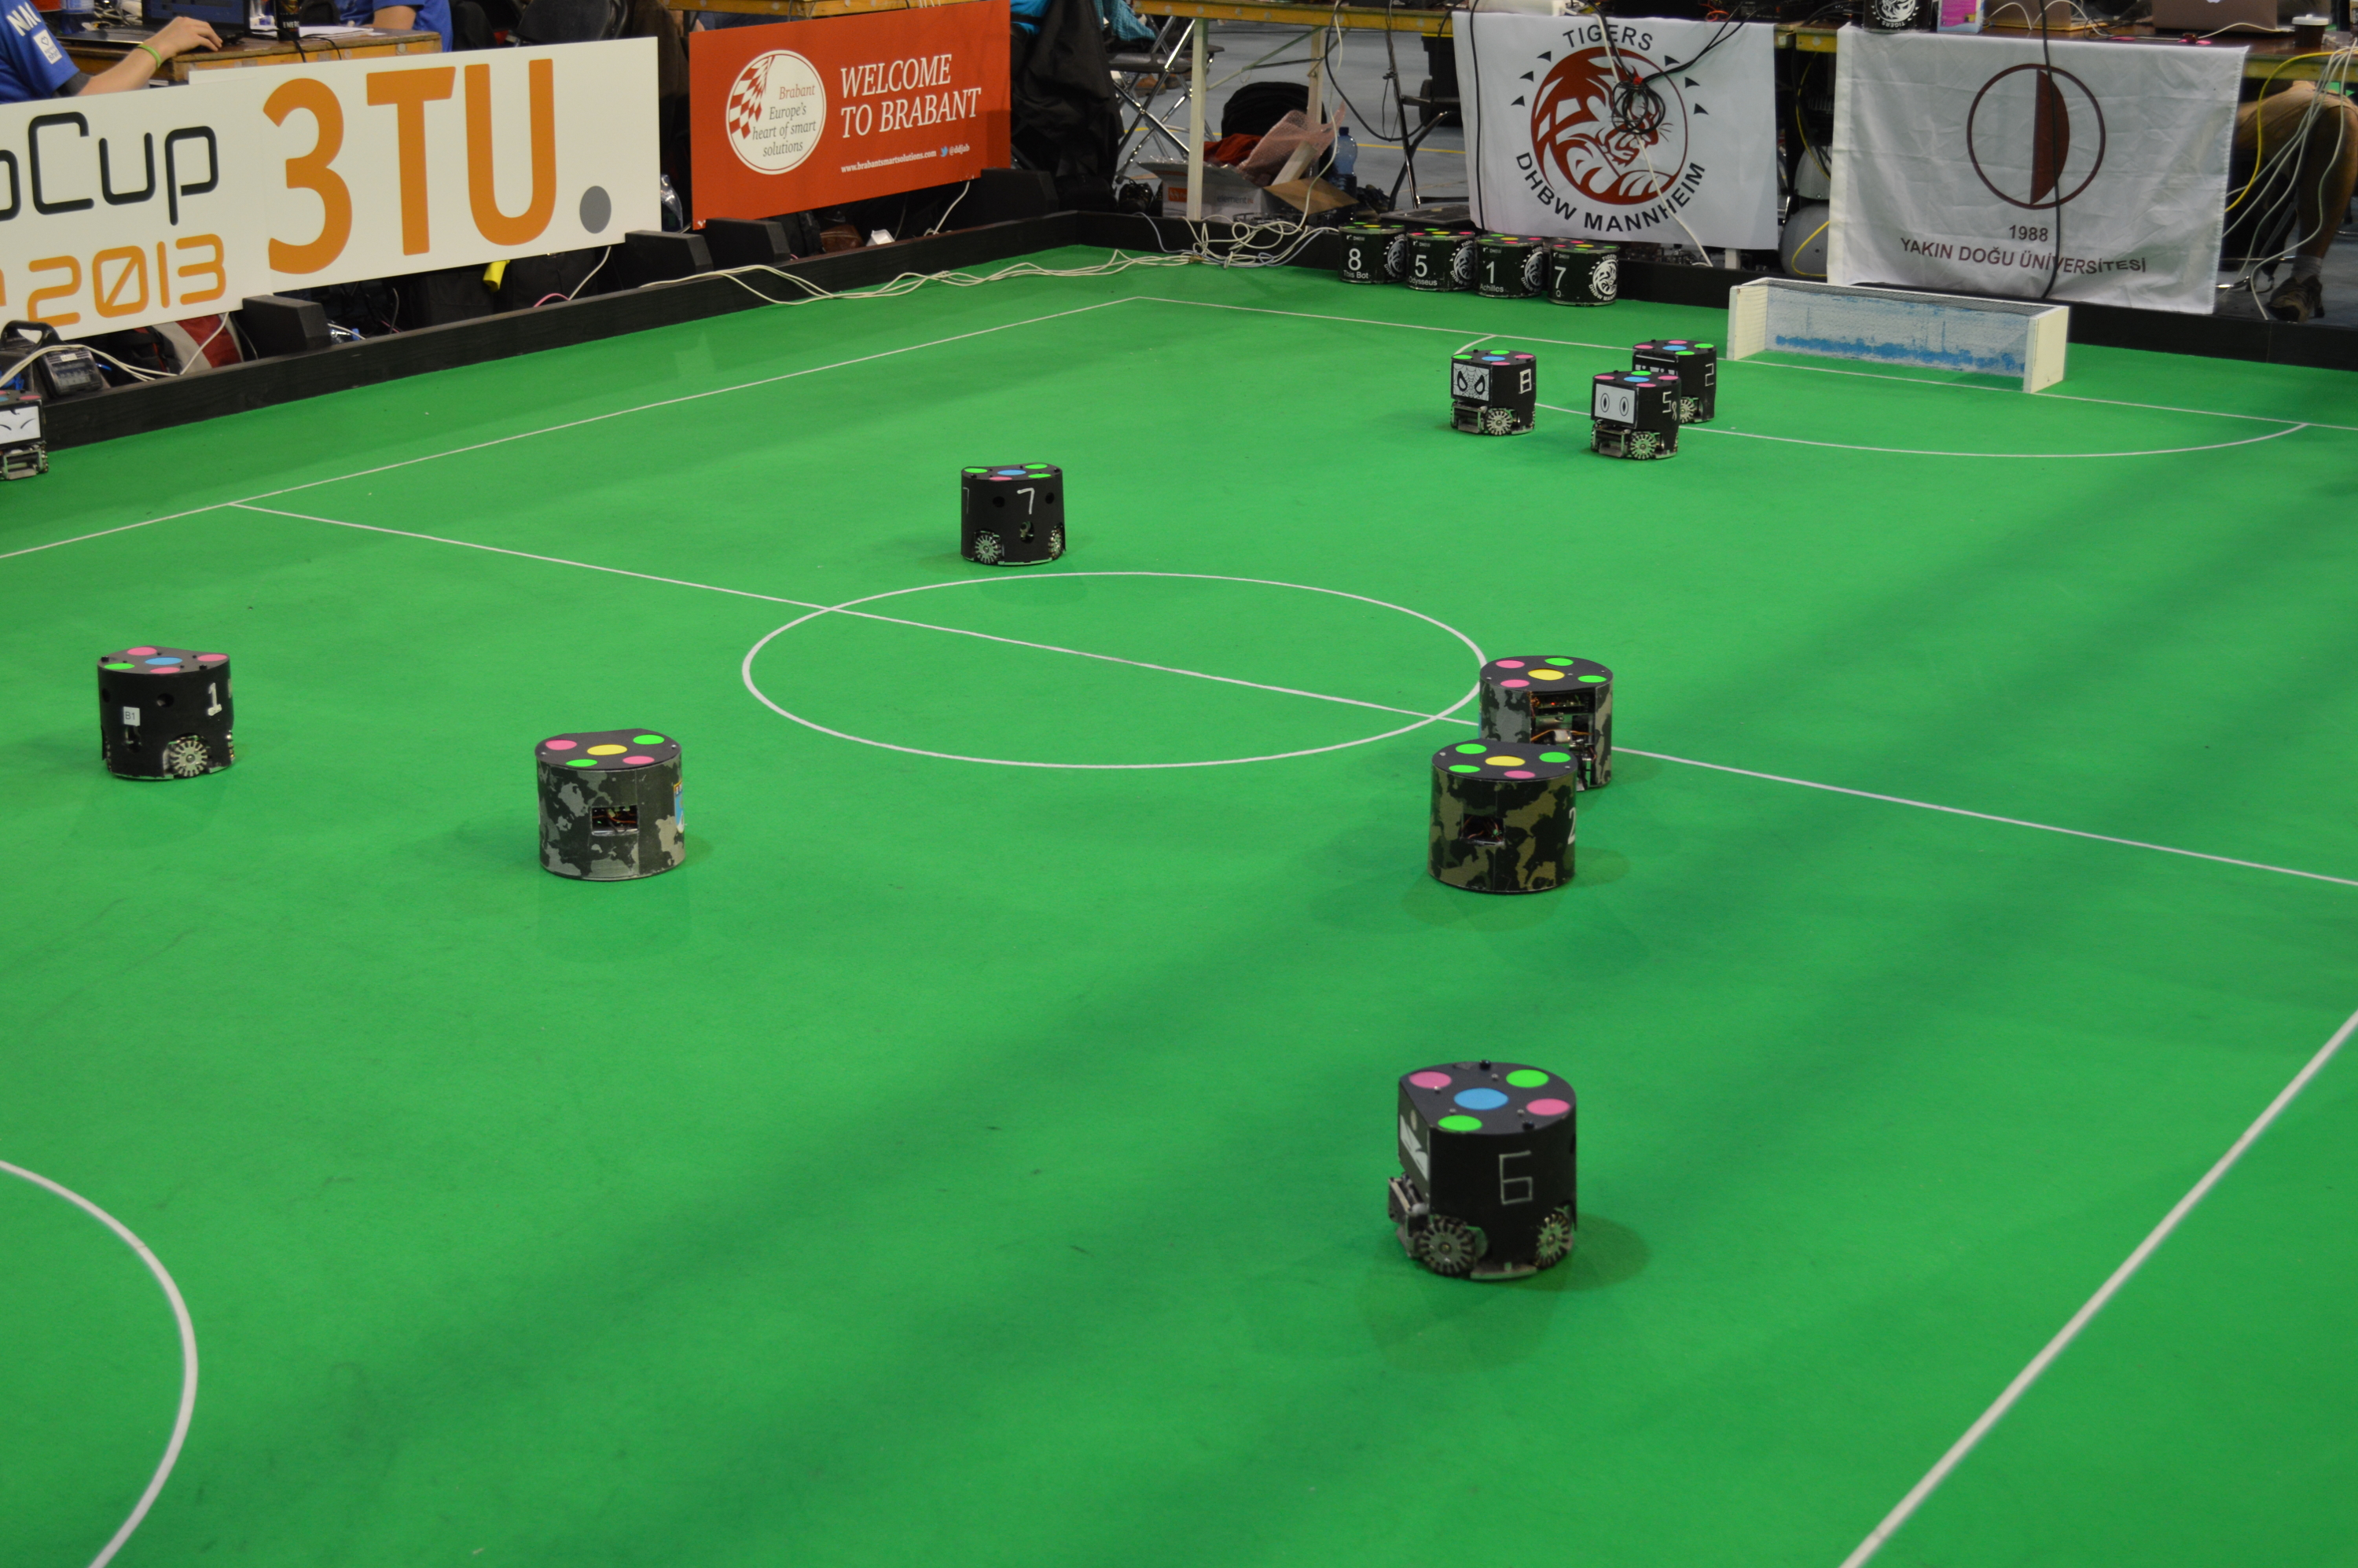
\includegraphics[width=0.8\linewidth]{robocup2013}
  \caption{Imagem da SSL \textit{RoboCup} 2013 em Eindhoven, na Holanda}\label{fig:robocup2013}
\end{figure}

Devido a alta complexidade desses ambientes, não é viável o planejamento
considerando diretamente as leis físicas. Como consequência, limita-se as ações
possíveis do robô no modelo utilizado no planejamento para que se possa simular
mais situações em tempo hábil, uma vez que o ambiente está continuamente sujeito
a modificações. Entretanto, para que as simulações sejam válidas, o robô real
deve estar em sintonia com seu modelo. Com efeito, o robô real deve executar os
comandos conforme o robô simulado, caso o mesmo ambiente simulado seja
encontrado na prática.

A ideia de robôs jogando futebol foi mencionada pela primeira vez pelo professor
Alan Mackworth (University of British Columbia, Canadá) em um artigo intitulado
"On Seeing Robots", apresentado no Vision Interface 92 e posteriormente
publicado em um livro chamado Computer Vision: System, Theory and Applications
\cite{basu1993computer}.  Independentemente, um grupo de pesquisadores japoneses
organizou um Workshop no Ground Challenge in Artificial Intelligence, em Outubro
de 1992, Tóquio, discutindo e propondo problemas que representavam grandes
desafios.
Esse Workshop os levou a sérias discussões sobre usar um jogo de futebol para
promover ciência e tecnologia. Estudos foram feitos para analisar a viabilidade
dessa ideia. Os resultados desses estudos mostram que a ideia era viável,
desejável e englobava diversas aplicações práticas. Em 1993, um grupo de
pesquisadores, incluindo Minoru Asada, Yasuo Kuniyoshi e Hiroaki Kitano,
lançaram uma competição de robótica chamada de Robot J-League (fazendo uma
analogia à J-League, nome da Liga Japonesa de Futebol Profissional). Em um mês,
vários pesquisadores já se pronunciavam dizendo que a iniciativa deveria ser
estendida ao âmbito internacional. Surgia então, a Robot World Cup Initiative
(RoboCup).

RoboCup é uma competição destinada a desenvolver os estudos na área de robótica
e Inteligência Artificial (IA) por meio de uma competição amigável. Além disso,
ela tem como objetivo, até 2050, desenvolver uma equipe de robôs humanóides
totalmente autônomos capazes de derrotar a equipe campeã mundial de futebol
humano. A competição possui várias modalidades. Neste trabalho, será analisada a
Small Size Robot League (SSL), também conhecida como F180. De acordo com as
regras da SSL de 2015, as equipes devem ser compostas por 6 robôs, sendo um deles o
goleiro, que deve ser designado antes do início do jogo. Durante o jogo, nenhuma
interferência humana é permitida com o sistema de controle dos robôs. É
fornecido aos times um sistema de visão global e esses controlam seus robôs através de
máquinas próprias. O sistema de controle dos robôs geralmente é externo e recebe
os dados de um conjunto de duas câmeras localizadas acima do campo. Esse sistema
de controle processa os dados, determina qual comando deve ser executado por
cada robô e envia este comando através de ondas de rádio aos robôs.
% Embora seja permitido que as equipes utilizem sistemas próprios de visão, a
% maioria das equipes utiliza a visão centralizada.

\section{Motivação}

% TODO: ABRIR AQUI UMA SUBSEÇÃO DENOMINADA CONTEXTUALIZAÇÃO INICIAL E COLOCAR AS
%       SEÇÕES 2.1 E 2.2 CO IP COMO SUBITENS. ?????

O futebol de robôs, problema padrão de investigação internacional, reúne grande
parte dos desafios presentes em problemas do mundo real a serem resolvidos em
tempo real. As soluções encontradas para o futebol de robôs podem ser
estendidas, possibilitando o uso da robótica em locais de difícil acesso para
humanos, ambientes insalubres e situações de risco de vida iminente.  Há
diversas novas áreas de aplicação da robótica, tais como exploração espacial e
submarina, navegação em ambientes inóspitos e perigosos, serviço de assistência
médica e cirúrgica, além do setor de entretenimento. Essas áreas podem ser
beneficiadas com o desenvolvimento de sistemas multi robôs. Nestes domínios de
aplicação, sistemas de multi robôs deparam-se sempre com tarefas muito difíceis
de serem efetuadas por um único robô.  Um time de robôs pode prover redundância
e contribuir cooperativamente para resolver o problema em questão. Com efeito,
eles podem resolver o problema de maneira mais confiável, mais rápida e mais
econômica, quando comparado com o desempenho que único robô teria.

Devido a alta complexidade de sistemas multiagentes dinâmicos, torna-se
necessário um modelo simplificado para que sejam executadas o maior número de
simulações possível.  Caso seja possível uma discretização, ter-se-á um número
finito de casos para serem avaliados. Com isso, pode-se desenvolver um sistema
multi-agente baseado em utilidade. Assim, o computador passa a escolher parte
da estratégia com base na função utilidade escolhida.
%como o Minimax (discutido no Capítulo~\ref{cap:minimax}) para encontrar
%soluções ao problema.

Isso é mais desejável que um modelo heurístico de IA, onde as soluções são
criadas com base nos ambientes identificados pelos modeladores. Isso, pois a
modelagem puramente heurística limita o número de jogadas que se pode executar e
limita a capacidade que o computador tem de testar um grande número de possibilidades.
O resultado é que a qualidade das jogadas se limita a capacidade de quem cria as
heurísticas.

\section{Objetivo}

O objetivo deste trabalho é desenvolver uma ferramenta de representação
comportamental baseado em otimização para futebol de robôs.
%O objetivo deste trabalho é desenvolver um algoritmo de controle para o futebol
%de robôs que obtenha um desempenho melhor que o utilizado atualmente, de acordo
%com a performance em um conjunto de partidas.
A meta intermediária é criar um modelo discreto sequencial
para o problema do futebol de robôs. A partir desta
discretização, foi desenvolvida uma arquitetura de controle
que seleciona jogadas o mais próximas da jogada ótima possível,
de acordo com uma função de avaliação e dentro do tempo disponível
para o planejamento.

\section{Justificativa}
% TODO: incluir referências

Uma arquitetura de controle que simule os diversos ambientes dinamicamente de
maneira sequencial de um ambiente multiagente permite que várias jogadas sejam
criadas dinamicamente, diferentemente de uma arquitetura estática baseada somente
em heurística. Essa abordagem heurística é legada da maneira como estratégias
são planejadas nos times de futebol humano.

Com tal mecanismo é possível melhorar a IA em uso pela RoboIME para tomar
decisões que levem a resultados melhores e, como consequência, ganhar mais
partidas. Nenhuma equipe atualmente esta seguindo esta abordagem, mas os autores
acreditam que essa é uma linha de pesquisa promissora, já que se utiliza da
capacidade que o computador tem de simular várias possibilidades em um curto
intervalo de tempo.

\section{Metodologia}

Para atingir os objetivos propostos será seguida a seguinte metodologia.
Inicialmente é criado um modelo sequencial do problema do futebol de robôs.
Para isso, a arquitetura do futebol de robôs considerada neste trabalho é
detalhada, juntamente com definições de termos relevantes para este trabalho.
% TODO: Mostrar os passos do trabalho, e não do relatório
%
%Um modelo abstrato do futebol de robôs é proposto para simplificar o problema
%e permitir que sejam feitas várias simulações durante o planejamento das
%jogadas. A função de avaliação, essecial para a seleção das jogas, é detalhada.
%
%Posteriormente a arquitetura da ferramenta a ser construida é apresentada.
%Os diversos componentes do sistema são detalhados.
%
%Em seguida, os resultados experimentais obtidos com a ferramenta detalhada
%anteriormente são apresentados.
%
%São apresentadas sugestões para trabalhos futuros e as principais dificuldades
%enfrentadas pelos autores são destacadas.
%
%Finalmente são apresentadas as conclusões do projeto.

\section{Estrutura}

% modelagem
No Capítulo~\ref{cap:modelagem}, um modelo do futebol de robôs é proposto.
Também é apresentada a função de avaliação.

% arquitetura
No Capítulo~\ref{cap:arquitetura}, a ferramenta proposta é desenvolvida com
base no modelo proposto anteriormente.

% resultados
No Capítulo~\ref{cap:resultados}, são apresentados os resultados obtidos
neste trabalho.

% considerações finais
No Capítulo~\ref{cap:cons_finais}, são apresentadas sugestões para trabalhos
futuros e as principais dificuldades enfrentadas pelos autores são destacadas.

% conclusao
Finalmente, são apresentados os principais resultados atingidos neste trabalho.

% vim: tw=80 et ts=2 sw=2 sts=2 ft=tex


% FIXME: FALTOU A SEÇÃO DE REVISÃO DE LITERATURA???

% Desenvolvimento
% ---------------

\section{Modelagem}\label{cap:modelagem}

Neste capítulo é criado um modelo sequêncial do problema do futebol de robôs. 
Para isso, a arquitetura do futebol de robôs considerada neste trabalho é
detalhada, juntamente com definições de termos relevantes para este trabalho.
Um modelo abstrato do futebol de robôs é proposto para simplificar o problema
e permitir que sejam feitas várias simulações durante o planejamento das
jogadas. A função de avaliação, utilizada para converter as jogadas em números,
é especificada.

\chapter{Arquitetura do Sistema}\label{cap:arquitetura}

Este capítulo descreve como a ferramenta desenvolvida interage com os
\textit{softwares} em uso na competição.

Os seguintes \textit{softwares} externos são de relevância para o entendimento
da arquitetura escolhida:

\begin{itemize}
  \item ssl-vision: desenvolvido pela comunidade e de uso oficial na competição
    para processamento das imagens da câmera nas partidas e distribuição pela
    rede dos dados processados (estado do jogo);
  \item grSim: desenvolvido pela comunidade e amplamente usado pelas equipes
    para simular o ambiente das partidas, o protocolo usado para enviar o estado
    pela rede é identico ao do ssl-vision;
  \item pyroboime: também chamado de core desenvolvido pela RoboIME, atualmente
    provê uma camada de abstração sobre a comunicação com o ambiente de jogo
    (real ou simulado) incluindo redução de ruído, planejamento de trajetória e
    controle.
\end{itemize}

Para fins práticos o desenvolvimento ocorre com validações no simulador (grSim).
O comportamento é compatível com as partidas oficiais.

\section{Comunicação com Componentes Externos}

\begin{figure}[H]
  \centering
  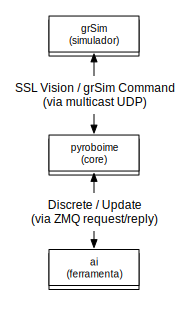
\includegraphics[height=10cm]{communication}
  \caption{Diagrama de comunicação entre os componentes.}\label{fig:arch-comm}
\end{figure}

A figura~\ref{fig:arch-comm} representa como os componentes se comunicam.  A
ferramenta se comunica apenas com o pyroboime para aproveitar todas as
funcionalidades necessárias que fogem ao escopo desse trabalho.  Por isso o foco
do desenvolvimento está concentrado em atender diretamente os objetivos.

As mensagens trocadas entre a ferramenta e o core (\textit{pyroboime}) é
codificada com o \textit{Protobuf}, uma biblioteca bem estabelecida que também é
usada nos protocolos oficiais da competição.  Desse modo o \textit{overhead} de
comunicação é baixo, não é necessário introduzir uma dependência ou codificação
manual no core e é possível que versões futuras sejam retrocompatíveis.

São dois tipos de mensagens:

\begin{itemize}
  \item atualização do estado: sentido do core para a ferramenta, codificadas
    com a mensagem UpdateMessage, descreve todas as informações necessárias para
    criar um estado novo;
  \item comando de ações: sentido ferramenta para o core, codificadas com a
    mensagem CommandMessage, descreve a ação que cada agente (robô) deve
    realizar.
\end{itemize}

As especificações de ambas as mensagens se encontram no anexo~\ref{att:protos}.

As mensagens são transmitidas num socket ZMQ (\textit{ZeroMQ}, uma biblioteca de
transmissão de dados na rede) visando a extensibilidade da ferramenta, pois com
tal biblioteca é possível distribuir mensagens entre vários nós de forma
confiável (característica desejável para um sistema distribuido) além de provêr
confiabilidade e auto-reconexão para o uso atual.

O modo de transmissão é \textit{request-reply} em que a ferramente age como
servidor respondendo as requisições do core, que consistem em atualizações cuja
a resposta deve ser o comando a ser executado naquele estado requisitado.  Na
prática a ferramenta irá transmitir o comando mais recente, que se encontra em
seu \textit{buffer}, descrito brevemente no seção~\ref{sec:threads}.

\section{\textit{Threads} do Sistema}\label{sec:threads}

\begin{figure}[H]
  \centering
  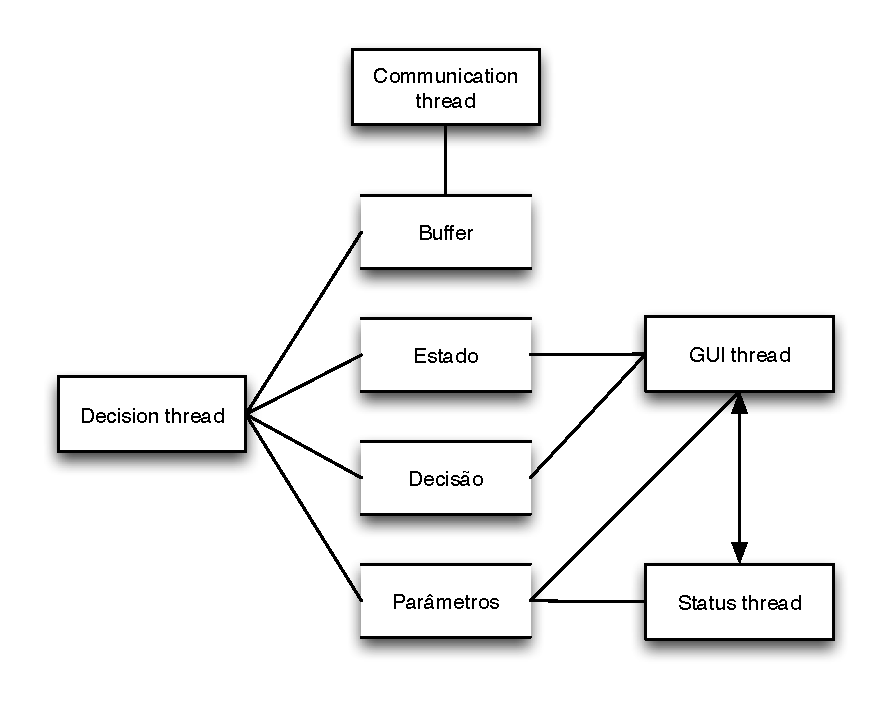
\includegraphics[height=10cm]{threads}
  \caption{Diagrama de relação entre \textit{threads} e
  dados.}\label{fig:arch-threads}
\end{figure}

A ferramenta está implementada em 4 \textit{threads} fixas de acordo com a
figura~\ref{fig:arch-threads}.  A separação foi motivada por:

\begin{itemize}
  \item A interface gráfica necessitar ser responsiva ao usuário;
  \item A taxa de tomada de decisão poder ser mais lenta que a taxa de
    atualização do estado, portanto a comunicação tem sua própria
    \textit{thread} que escreve e lê de um buffer compartilhado pela
    \textit{thread} de tomada de decisão;
  \item Certas informações devem ser coletadas periódicamente para atualizar
    alguns parâmetros e exibidas para o usuário.
\end{itemize}

\section{API Pública}

% TODO: um diagrama de colaboração de classes seria útil aqui

Uma API consiste nas estruturas e funções (ou também métodos) que estão
disponíveis para o programador.  A ferramenta está programada de forma que
também é possível fazer o uso programático de suas funcionalidades.

Esta seção descreve com detalhes cada estrutura e função presente na API da
ferramenta.  É um objetivo desta seção documentar o código da ferramenta para
possibilitar a evolução dessa em projetos futuros ou integração em outros
projetos.

Todas as estruturas e funções estão expostas em \textit{headers} C++, porém esta
documentação irá tratar apenas das funcionalidades e organização sem prender à
sintaxe ou modo de uso na linguagem em que está programada.  Para tais detalhes
o anexo~\ref{att:headers} pode ser consultado, esse contém o conteúdo dos
headers tratados nesta seção.

\subsection*{Enumeração \textit{ActionType}}

Representa o tipo da ação.

\subsubsection*{Alternativas}

\begin{itemize}
  \item \textit{NONE}: nenhuma ação;
  \item \textit{MOVE}: acão de movimentação;
  \item \textit{PASS}: ação de passe;
  \item \textit{KICK}: ação de chute.
\end{itemize}

\subsection*{Estrutura \textit{Action}}

Representa a ação individual a ser executada por um robô, não está amarrada à um
robô, essa associação deve ser feita pelo usuário da estrutura, isso permite uma
associação implicita baseada na ordem do vetor ou outros tipos de otimizações,
por esse motivo algumas funções recebem um Id de robô para saber qual robô usar
em certas circunstâncias.

\subsubsection*{Atributos}

\begin{itemize}
  \item \textit{type}: tipo (\textit{ActionType}), por padrão é do tipo NONE;
  \item \textit{move_pos}: posição destino da movimentação;
  \item \textit{kick_pos}: posição alvo do chute;
  \item \textit{pass_receiver}: Id do robô que deve receber o passe.
\end{itemize}

\subsubsection*{Métodos}

\begin{itemize}
  \item \textit{make_move_action}
    \par Entrada: vetor indicando um destino.
    \par Saída: ação do tipo MOVE.
  \item \textit{make_kick_action}
    \par Entrada: vetor indicando um alvo.
    \par Saída: ação do tipo KICK.
  \item \textit{make_pass_action}
    \par Entrada: Id de robô, que irá receber o passe.
    \par Saída: ação do tipo PASS.
  \item \textit{gen_move_action}
    \par Entrada: Id de um robô, estado, tabela de decisão.
    \par Saída: ação do tipo MOVE aleatória, que não colide com a posição de
    nenhum outro robô, nem com a posição destino desses de acordo com a tabela
    de decisão.
  \item \textit{gen_kick_action}
    \par Entrada: Id de um robô, estado, tabela de decisão.
    \par Saída: ação do tipo KICK no ponto de maior abertura do gol do inimigo
    que continuar aberto após as movimentações da tabela de decisão.  É assumido
    que um chute é possível e isso foi verificado previamente.
  \item \textit{gen_pass_action}
    \par Entrada: Id de um robô, estado, tabela de decisão.
    \par Saída: ação do tipo PASS aleatória para algum robô (do mesmo time) que
    possa receber o passe, o critério para receber o passe envolve que o
    receptor chegue em seu destino antes que o passador consiga chegar na bola e
    chuta-lá até o destino do receptor, além disso após o chute o receptor deve
    conseguir ser o dono da bola.
  \item \textit{gen_primary_action}
    \par Entrada: Id de um robô, estado, tabela de decisão, flag que indica se é
    de chute.
    \par Saída: ação do tipo KICK ou PASS, simplesmente abstrai
    \textit{gen_pass_action} ou \textit{gen_kick_action} para evitar verbosidade.
  \item \textit{apply_to_state}
    \par Entrada: ação, Id do robô, referência para um estado.
    \par Efeito: aplica a ação a um estado.  É assumido que a ação pode ser
    aplicada.  Ações de chute levam a bola para o gol.
\end{itemize}

%#ifndef CONSTS_H
%#define CONSTS_H
%
%constexpr int N_ROBOTS = 6;
%constexpr int MAX_SUGGESTIONS = 30;
%constexpr int MAX_SUGGESTION_SPOTS = 30;
%
%// Units are SI: m, m/s, s, ...
%
%constexpr float LINE_WIDTH = 0.010;
%constexpr float FIELD_WIDTH = 8.090;
%constexpr float FIELD_HEIGHT = 6.050;
%constexpr float GOAL_WIDTH = 1.000;
%constexpr float GOAL_DEPTH = 0.180;
%constexpr float GOAL_WALL_WIDTH = 0.020;
%constexpr float CENTER_CIRCLE_RADIUS = 0.500;
%constexpr float DEFENSE_RADIUS = 1.000;
%constexpr float DEFENSE_STRETCH = 0.500;
%constexpr float BOUNDARY_WIDTH = 0.500;
%constexpr float REFEREE_WIDTH = 0.250;
%constexpr float ROBOT_RADIUS = 0.180 / 2;
%constexpr float BALL_RADIUS = 0.043 / 2;
%constexpr float ROBOT_MAX_SPEED = 1.0;
%constexpr float ROBOT_KICK_SPEED = 6.0;
%constexpr float MAX_PASS_DISTANCE = 2.5;
%
%constexpr const char *PROGRAM_NAME =
%    "AI for RoboIME"; // TODO: better name maybe?
%constexpr int GUI_DEFAULT_WIDTH = 944;
%constexpr int GUI_DEFAULT_HEIGHT = 740;
%
%enum _ParamGroup {
%  MAX_ATTACK = 0,
%  MIN_ATTACK = 1,
%  MAX_CONQUER = 2,
%  MIN_CONQUER = 3
%};
%
%extern const int *const PARAM_GROUP;
%extern bool PARAM_GROUP_AUTOSELECT;
%extern bool PARAM_GROUP_CONQUER;
%extern float PARAM_GROUP_THRESHOLD;
%extern float PARAM_GROUP_CONQUER_TIME;
%void set_param_group(int new_param_group);
%
%#ifdef _CONST_IMPL
%#define PARAM(TYPE, NAME, DEFAULT) _CONST_IMPL(TYPE, NAME, DEFAULT)
%#else
%#define PARAM(TYPE, NAME, DEFAULT) extern TYPE NAME;
%#endif
%
%PARAM(bool, CONSTANT_RATE, true);
%PARAM(bool, KICK_IF_NO_PASS, false);
%PARAM(int, DECISION_RATE, 7);
%PARAM(int, RAMIFICATION_NUMBER, 5000);
%PARAM(int, FULL_CHANGE_PERCENTAGE, 100);
%PARAM(int, MAX_DEPTH, 0);
%PARAM(float, KICK_POS_VARIATION, 0.150);
%PARAM(float, MIN_GAP_TO_KICK, 18.0);
%PARAM(float, DESIRED_PASS_DIST, 2.0);
%PARAM(float, WEIGHT_BALL_POS, 0);
%PARAM(float, WEIGHT_MOVE_DIST_MAX, 0);
%PARAM(float, WEIGHT_MOVE_DIST_TOTAL, 0);
%PARAM(float, WEIGHT_MOVE_CHANGE, 2);
%PARAM(float, WEIGHT_PASS_CHANGE, 2);
%PARAM(float, WEIGHT_KICK_CHANGE, 2);
%PARAM(float, TOTAL_MAX_GAP_RATIO, 0.5);
%PARAM(float, WEIGHT_CLOSE_TO_BALL, 1000);
%PARAM(float, WEIGHT_ENEMY_CLOSE_TO_BALL, 1000);
%PARAM(float, WEIGHT_HAS_BALL, 5000);
%PARAM(float, WEIGHT_ATTACK, 1000);
%PARAM(float, WEIGHT_SEE_ENEMY_GOAL, 10);
%PARAM(float, WEIGHT_BLOCK_GOAL, 180);
%PARAM(float, WEIGHT_BLOCK_ATTACKER, 5000);
%PARAM(float, WEIGHT_GOOD_RECEIVERS, 0);
%PARAM(float, WEIGHT_RECEIVERS_NUM, 20);
%PARAM(float, WEIGHT_ENEMY_RECEIVERS_NUM, 20);
%PARAM(float, DIST_GOAL_PENAL, 2000);
%PARAM(float, DIST_GOAL_TO_PENAL, 1.0);
%PARAM(float, MOVE_RADIUS_0, 0.5);
%PARAM(float, MOVE_RADIUS_1, 2.0);
%PARAM(float, MOVE_RADIUS_2, 7.0);
%
%enum Weight {
%  _WEIGHT_BALL_POS,
%  _WEIGHT_MOVE_DIST_MAX,
%  _WEIGHT_MOVE_DIST_TOTAL,
%  _WEIGHT_MOVE_CHANGE,
%  _WEIGHT_PASS_CHANGE,
%  _WEIGHT_KICK_CHANGE,
%  _WEIGHT_CLOSE_TO_BALL,
%  _WEIGHT_ENEMY_CLOSE_TO_BALL,
%  _WEIGHT_HAS_BALL,
%  _WEIGHT_ATTACK,
%  _WEIGHT_SEE_ENEMY_GOAL,
%  _WEIGHT_BLOCK_GOAL,
%  _WEIGHT_BLOCK_ATTACKER,
%  _WEIGHT_GOOD_RECEIVERS,
%  _WEIGHT_RECEIVERS_NUM,
%  _WEIGHT_ENEMY_RECEIVERS_NUM,
%  _WEIGHT_PENALS,
%  W_SIZE
%};
%
%#ifndef _CONST_IMPL
%#undef PARAM
%#endif
%
%#endif

\subsection*{Estrutura \textit{Decision}}

Representa uma decisão total de um time, isto é todos os robôs irão possuir
ações, mesmo que sejam do tipo NONE.  Similarmente à uma ação individual, uma
decisão não está atrelada a um time, e por isso é comum alguns métodos
precisarem de uma decisão e o time a qual será aplicada.

\subsubsection*{Atributos}

\begin{itemize}
  \item \textit{action}: array de ações de tamanho igual ao número de robôs que
    um time possui.
\end{itemize}

\subsubsection*{Métodos}

\begin{itemize}
  \item \textit{apply_to_state}
    \par Entrada: decisão, time e referência a um estado.
    \par Efeito: todas as ações da decisão são aplicadas ao estado, assim como
    em uma ação é assumido que é possível aplicar a decisão.
  \item \textit{gen_decision}
    \par Entrada: flag que indica se é chute, estado, jogador, tabela de decisão
    e robô que irá se movimentar (opcional)
    \par Saída: decisão gerada aleatoriamente usando as restrições de geração de
    ações.  Caso um robô para se movimentar seja especificado esse será o único
    a receber uma movimentação aleatória os outros seguirão com as ações da
    tabela de decisão.
  \item \textit{to_proto_command}
    \par Entrada: decisão, time, referência para um mensagem
    \textit{CommandMessage}, tabela de Ids.
    \par Efeito: converte uma decisão para a estrutura de mensagem gerada pelo
    \textit{Protobuf}.
\end{itemize}

\subsection*{Enumeração \textit{DecisionSource}}

Representa de qual tipo de ramo uma decisão foi gerada.

\subsubsection*{Alternativas}

\begin{itemize}
  \item \textit{NO_SOURCE}: não há fonte, usado como padrão para decisões
    vazias.
  \item \textit{SUGGESTION}: decisão gerada a partir de uma sugestão (posição
    chave).
  \item \textit{TABLE}: decisão gerada a partir de uma tabela de decisão.
  \item \textit{FULL_RANDOM}: decisão gerada a partir de uma movimentação de
    todos os robôs.
  \item \textit{SINGLE_RANDOM}: decisão gerada a partir da movimentação de um
    único robô.
\end{itemize}

\subsection*{Estrutura \textit{DecisionTable}}

\subsubsection*{Atributos}

\begin{itemize}
  \item \textit{kick_robot}: Id do robô com ação de chute, é opcional, na
    ausência indica que não há robo com ação de chute.
  \item \textit{kick}: ação de chute.
  \item \textit{pass_robot}: Id do robô com ação de chute, é opcional, na
    ausência indica que não há robo com ação de chute.
  \item \textit{pass}: ação de passe.
  \item \textit{move}: array de ações de movimentação com tamanho igual ao
    número de robôs que um time possui.
\end{itemize}

%#ifndef DRAW_H
%#define DRAW_H
%
%#include "player.h"
%
%void screen_zoom(int width, int height, double zoom, double center_x,
%                 double center_y);
%void draw_state(const struct State &state);
%void draw_decision(const struct Decision &decision,
%                   const struct State &state, Player player);
%void draw_suggestion(const struct SuggestionTable &table);
%void draw_app_status(void);
%void draw_options_window(void);
%
%#endif

%#ifndef FILTER_H
%#define FILTER_H
%
%#include "array.h"
%
%// this is a exclusion filter, true means out
%// (rationale behind it is that default initialization goes to no
%// filter)
%struct TeamFilter : TeamArray<bool> {
%  int count = N_ROBOTS;
%};
%
%void filter_out(TeamFilter &team_filter, int i);
%
%#endif

\subsection*{Estrutura \textit{Optimization}}

Uma instância representa uma unidade de otimização.  A princípio seria
necessário apenas uma função otimizadora mas com existe persistência de
informações (como tabela de decisão) então foi criada essa estrutura para
persistir tais dados de maneira explícita.

\subsubsection*{Atributos}

\begin{itemize}
  \item \textit{table}: tabela de decisão.
  \item \textit{robot_to_move}: usado para fazer o rodízio do robô que irá ser
    movimentado no modo SINGLE_RANDOM.
  \item \textit{table_initialized}: flag para marcar se a tabela já foi
    inicializada, usado apenas para algumas otimizações.
\end{itemize}

\subsection*{Métodos}

\begin{itemize}
  \item \textit{decide}
    \par Entrada: instância de otimização, estado, time, sugestões (opcional)
    \par Saída: decisão valorada, número de ramificação (opcional)
\end{itemize}

\subsection*{Enumeração \textit{Player}}

Indica um time.

\subsubsection*{Alternativas}

\begin{itemize}
  \item \textit{MIN}: time cujo valor é minimizado, normalmente configurado como
    time inimigo.
  \item \textit{MAX}: time cujo valor é maximizado.
\end{itemize}

\subsection*{Estrutura \textit{Segment}}

Representa um segmento de uma dimensão, usado para cálculo de \textit{gaps}
(vãos) no gol.

\subsubsection*{Atributos}

\begin{itemize}
  \item \textit{u}: valor superior (up).
  \item \textit{d}: valor inferior (down).
\end{itemize}

\subsection*{Estrutura \textit{State}}

Representa o estado do jogo.  É importante ressaltar que os Ids usados dentro da
ferramenta têm significado diferente do Id usado no jogo.  Aqui os Ids são
únicos para cada robô, mesmo entre times, isto é, um Id usado pelo time MIN não
pode ser usado pelo time MAX.  Mais notável é que os Ids variam necessáriamente
entre $0$ e $11$ inclusive, sendo a primeira porção correspondente ao time MIN e
a segunda ao time MAX.  Esse design permite usar Ids como índices de arrays e
determinar o time a partir de um Id.  Para tanto é necessário uma tabela de Ids
para mapear para os Ids usados na partida.

\subsubsection*{Atributos}

\begin{itemize}
  \item \textit{ball}: vetor posição da bola.
  \item \textit{ball_v}: vetor velocidade da bola.
  \item \textit{robots}: array de vetores posição de cada robô do jogo.
  \item \textit{robots_v}: array de vetores velocidade de cada robô do jogo.
\end{itemize}

\subsection*{Métodos}

\begin{itemize}
  \item \textit{uniform_rand_state}
    \par Saída: estado uniformemente aleatório, usado apenas para testes.
  \item \textit{can_kick_directly}
    \par Entrada: estado, time.
    \par Saída: booleano, se o time é capaz de realizar um chute direto.
  \item \textit{robot_with_ball}
    \par Entrada: estado.
    \par Saída: Id do robô com a bola.
    \par Saídas opcionais: tempo para o time MIN alcançar a bola, tempo para o
    time MAX alcançar a bola, Id do robô do time MIN mais próximo à bola, Id do
    robô do time MAX mais próximo à bola.
    \par A posse de bola usa o tempo para chegar à bola, que leva em
    consideração a velocidade da bola.
  \item \textit{total_gap_len_from_pos}
    \par Entrada: estado, posição origem, time, robô a ser ignorado (opcional).
    \par Saída: soma de todas as aberturas vistas a partir da origem no gol do
    time especificado.
  \item \textit{max_gap_len_from_pos}
    \par Entrada: estado, posição origem, time, robô a ser ignorado (opcional).
    \par Saída: maior entre todas as aberturas vistas a partir da origem no gol do
    time especificado.
  \item \textit{time_to_pos}
    \par Entrada: vetor posição da origem, vetor velocidade da origem, vetor posição
    do destino, vetor velocidade do destino, velocidade máxima do ponto de
    origem (opcional, por padrão do robô).
    \par Saída: menor tempo para o ponto chegar da origem no destino assumindo
    aceleração infinita do ponto e velocidade constante do destino.
  \item \textit{discover_gaps_from_pos}
    \par Entrada: estado, posição de origem, jogador, robô a ser ignorado
    (opcional).
    \par Saída: array de segmentos e tamanho do array, contém todos os segmentos
    que representam os vãos (gaps) que podem ser observados no gol do time
    especificado.
  \item \textit{evaluate_with_decision}
    \par Entrada: time, estado, decisão, tabela de decisão.
    \par Saída: valor, valores individuais por peso (opcional)
    \par Essa é a função objetivo.
  \item \textit{discover_possible_receivers}
    \par Entrada: estado, tabela de decisão, jogador, Id do robô que faz o
    passe.
    \par Saída: lista dos robôs to time dado que podem receber passes.
  \item \textit{update_grom_proto}
    \par Entrada: referência para um estado, mensagem UpdateMessage, tabela de
    Ids.
    \par Efeito: atualiza o estado com os dados da mensagem se baseando no
    mapeamento da tabela de Ids.
\end{itemize}

\subsection*{Estrutura \textit{SuggestionTable}}

Tabela de sugestão, também referida por Posições Chaves.  Representa um conjunto
de posições chaves que é usado para gerar uma única decisão.

\subsubsection*{Atributos}

\begin{itemize}
  \item \textit{name}: nome do conjunto, útil para rótulos como 'barreira' ou
    '2-2-1' ou 'ataque pela direita'.
  \item \textit{spots_count}: contagem de posições.
  \item \textit{spots}: array de vetores posição.
  \item \textit{usage_count}: contagem de uso desta tabela, usado para
    estatísticas.
\end{itemize}

\subsubsection*{Métodos}

\begin{itemize}
  \item \textit{add_spot}
    \par Entrada: tabela de sugestão.
    \par Saída: novo tamanho da tabela, ou $-1$ em caso de erro.
    \par Efeito: adiciona uma posição na tabela.
  \item \textit{del_spot}
    \par Entrada: tabela de sugestão, posição a remover.
    \par Saída: novo tamanho da tabela, ou $-1$ em caso de erro.
  \item \textit{gen_decision}
    \par Entrada: flag indicando se decisão é de chute, tabela de sugestão,
    estado, tabela de decisão, time.
    \par Saída: decisão construída a partir da tabela de sugestão, o
    comportamento há menos posições que robôs é preencher com moves aleatórios e
    quando há mais posiçoes que robôs é usar as posições mais próximas há cada
    robô sem que haja repetição.
\end{itemize}

\subsection*{Estrutura \textit{Suggestions}}

Representa o conjunto de todas as tabelas de sugestões.

\subsubsection*{Atributos}

\begin{itemize}
  \item \textit{tables}: tabelas de sugestão.
  \item \textit{tables_count}: contagem de tabelas.
  \item \textit{last_use}: posição da última tabela usada para gerar uma decisão.
\end{itemize}

\subsubsection*{Métodos}

\begin{itemize}
  \item \textit{add_suggestion}
    \par Entrada: conjunto de sugestões.
    \par Saída: novo tamanho do conjunto, ou $-1$ em caso de erro.
    \par Efeito: adiciona uma posição no conjunto com uma tabela vazia.
  \item \textit{del_suggestion}
    \par Entrada: conjunto de sugestões, posição a remover.
    \par Saída: novo tamanho do conjunto, ou $-1$ em caso de erro.
  \item \textit{save_suggestions}
    \par Entrada: conjunto de sugestões, caminho de arquivo.
    \par Efeito: salva no arquivo o conjunto de sugestões em um formato textual.
  \item \textit{load_suggestions}
    \par Entrada: conjunto de sugestões, caminho de arquivo.
    \par Efeito: carrega do arquivo o conjunto de sugestões.
\end{itemize}

%#ifndef UTILS_H
%#define UTILS_H
%
%#include <cmath>
%
%#include "consts.h"
%#include "player.h"
%#include "vector.h"
%
%#define FOR_RANGE(I, F, T) for (int I = (F); I < (T); I++)
%#define FOR_N(I, N) FOR_RANGE(I, 0, N)
%#define FOR_N_IN(I, N, F) FOR_RANGE(I, 0, N) if (!F[I])
%#define FOR_EVERY_ROBOT(I) FOR_RANGE(I, 0, 2 * N_ROBOTS)
%#define FOR_TEAM_ROBOT(I, T)                                           \
%  FOR_RANGE(I, T *N_ROBOTS, (1 + T) * N_ROBOTS)
%#define FOR_EVERY_ROBOT_IN(I, F) FOR_EVERY_ROBOT(I) if (!F[I])
%#define FOR_TEAM_ROBOT_IN(I, T, F) FOR_TEAM_ROBOT(I, T) if (!F[I])
%
%constexpr int ROBOT_WITH_PLAYER(int R, Player P) {
%  return P * N_ROBOTS + R % N_ROBOTS;
%}
%
%constexpr Player ENEMY_FOR(Player P) { return P == MIN ? MAX : MIN; }
%constexpr Player PLAYER_OF(int R) {
%  return R / N_ROBOTS == MIN ? MIN : MAX;
%}
%constexpr Player ENEMY_OF(int R) { return ENEMY_FOR(PLAYER_OF(R)); }
%
%// 1 for MIN -1 for MAX
%constexpr int PLAYER_SIGN(Player P) { return P == MAX ? 1 : -1; }
%
%// XXX: MAX to the left, not taking into account that it may be
%// otherwise
%constexpr float GOAL_Y(Player) { return 0; }
%constexpr float GOAL_X(Player P) {
%  return -PLAYER_SIGN(P) * FIELD_WIDTH / 2;
%}
%constexpr Vector GOAL_POS(Player P) { return {GOAL_X(P), GOAL_Y(P)}; }
%
%// angle mesures conversions radians <-> degrees
%template <typename T> constexpr T RADIANS(T DEGREES) {
%  return M_PI * DEGREES / 180.;
%}
%template <typename T> constexpr T DEGREES(T RADIANS) {
%  return 180. * RADIANS / M_PI;
%}
%
%// a number squared
%template <typename T> constexpr T SQ(T X) { return X * X; }
%
%#endif

\subsection*{Estrutura \textit{ValuedDecision}}

Essa estrutura existe para anexar um valor à uma decisão, a intenção é que esse
seja um valor calculato pela função objetivo.  Uma alternativa seria usar tuplas
ou retornar o valor em um argumento de saída (pointeiro ou referência) mas a
estrutura é simples e possui uma semântica explícita e facilita evoluções, como
por exemplo a própria adição do attributo \textit{values}.

\subsubsection*{Atributos}

\begin{itemize}
  \item \textit{value}: valor associado à decisão.
  \item \textit{values}: array de valores que explicita quanto parcela da função
    objetivo contribui com o valor total, a soma dos valores será igual ao
    atributo \textit{value}.
  \item \textit{decision}: decisão associada ao valor.
\end{itemize}


\subsection*{Estrutura \textit{Vector}}

Vetor em duas dimensões usado para representar posições e velocidades no
programa.  Não deve ser confundido com um \textit{array}, que é uma sequência
de tamanho genérico (porém fixo) sem semântica associada.

\subsubsection*{Atributos}

\begin{itemize}
  \item \textit{x}: componente no eixo $x$.
  \item \textit{y}: componente no eixo $y$.
\end{itemize}

\subsubsection*{Métodos}

Alguns operadores foram definidos para essa estrutura de modo que suas operações
reflitam as operações matemáticas normalmente associadas a vetores.  Tais
operadores foram omitidos da lista de métodos mas podem ser consultados no
anexo~\ref{att:headers}.

\begin{itemize}
  \item \textit{norm2}
    \par Entrada: vetor.
    \par Saída: norma do vetor ao quadrado, usado para simplificar algumas
    operações, é ligeiramente menos custoso que a norma.
  \item \textit{norm}
    \par Entrada: vetor.
    \par Saída: norma do vetor.
  \item \textit{unit}
    \par Entrada: vetor.
    \par Saída: vetor com mesma direção porém norma unitária.
  \item \textit{uniform_rand_vector}
    \par Entrada: valor $r_x$, valor $r_y$.
    \par Saída: vetor aleatório distribuído uniformemente no região:
    $-r_x < x < r_x$, $-r_y < y < r_y$.
  \item \textit{normal_rand_vector}
    \par Entrada: vetor origem, valor sigma.
    \par Saída: vetor normalmente distribuído na origem e sigma entrados.
  \item \textit{rand_vector_bounded}
    \par Entrada: vetor origem, valor do raio, valores $r_x$ e $r_y$.
    \par Saída: vetor uniformemente distribuído em um círculo centrado na origem
    com o raio entrado que necessariamente está contido na região
    $-r_x < x < r_x$, $-r_y < y < r_y$, a segunda condição é sempre atendida nem
    que seja necessário quebrar a primeira.
  \item \textit{line_segment_cross_circle}
    \par Entrada: vetores $p_1$, $p_2$, vetor origem e valor do raio.
    \par Saída: verdadeiro se o segmento $(p_1, p_2)$ intercepta o círculo
    centrado na origem com o raio entrado.
  \item \textit{dist}
    \par Entrada: vetores $v_1$ e $v_2$.
    \par Saída: distância entre os vetores, sinônimo de $norm(v_1 - v_2)$.
\end{itemize}


% vim: tw=80 et ts=2 sw=2 sts=2 ft=tex

\section{Definições}\label{sec:defs}

\begin{defi}[Corpo Rígido]
  Um corpo rígido $cr$ é definido por dois subconjuntos disjuntos
  de parâmetros $cr= \langle \hat{cr}, \bar{cr} \rangle$ em que:
  \begin{itemize}
    \item $\hat{cr} = \langle pos, \theta, vel, \omega \rangle$,
    que são os parâmetros de estado mutáveis, respectivamente:
    posição ($\mathbb{R} ^{3}$), orientação ($\mathbb{R} ^{3}$),
    velocidade linear ($\mathbb{R} ^{3}$), velocidade angular
    ($\mathbb{R} ^{3}$)

    \item $\bar{cr} :$ parâmetros imutáveis do corpo que descrevem sua
    natureza fixa e que permanecem constantes ao longo do curso de 
    planejamento.
  \end{itemize}
\end{defi}

  Exemplos de parâmetros considerados nesta modelagem imutáveis são:
  coeficiente de atrito estático e dinâmico, descrição $3D$ do corpo
  (por exemplo, por meio de um conjunto de primitivas $3D$), centro de
  massa no referencial do corpo, coeficiente de restituição,
  coeficiente de amortecimento linear e angular.

\begin{defi}[Bola]\label{def:bola}
  Bola é um corpo rígido $b$, no qual somente as componentes
  $\langle x,y \rangle$ do parâmetro $\hat{b}.pos$ são
  observáveis.
\end{defi}

  De acordo com a arquitetura do jogo descrita na Seção~\ref{sec:arch_ssl},
  tem-se que, a partir de uma sequência
  de quadros, é possível obter um valor estimado para o parâmetro
  $\hat{b}.vel$ a partir do intervalo entre os dados recebidos
  da \textit{SSL-Vision} e da equação $ vel \approxeq 
  \frac{\Delta pos}{\Delta t} $. Entretanto, uma vez que a componente
  $z$ de $\hat{b}.pos$ não é observável, $\hat{b}.vel.z$ 
  não pode ser estimada a partir do intervalo entre os dados recebidos
  da \textit{SSL-Vision}. Semelhantemente,  uma vez que o
  parâmetro $\hat{b}.\theta$ também não pode ser observado,
  não se pode estimar o valor de $\hat{b}.\omega$ com exatidão.

% XXX[vbramigk] definir skill

\begin{defi}[Robô]
  Robô, representado por $r$, é um conjunto de sistemas compostos
  de corpos rígidos, \textit{hardware} e \textit{firmware}. Neste
  trabalho será considerado que o robô tem os seguintes sistemas:

  \begin{itemize}
    \item Drible: imprime um torque a bola;
    \item Chute baixo: imprime uma força à bola $b$
          e, possivelmente, um torque, com o objetivo de
          alterar as componentes $\langle x,y \rangle$
          do parâmetro $\hat{b}.vel$;
    \item Chute alto: imprime uma força à bola $b$
          e, possivelmente, um torque, com o objetivo de
          alterar as componentes $\langle x,y,z \rangle$
          do parâmetro $\hat{b}.vel$, com $\hat{b}.vel_z \neq 0$;
    \item Receptor: recebe comandos enviados pelo sistema de
          transmissão de seu respectivo time;
    \item Sistema de movimentação: imprime uma força e um torque
          ao centro de massa global do $r$;
  \end{itemize}
\end{defi}

  A Figura~\ref{fig:rob_data} ilustra os parâmetros de estado mutaveis
  do rôbo. Por meio dos sistemas listados acima, cada robô $r$ pode
  executar um conjunto de ações $A_{rob}$. A Figura~\ref{fig:robo}
  apresenta os atuadores típicos de um robô da SSL.

  \begin{figure}[H]
    \centering
    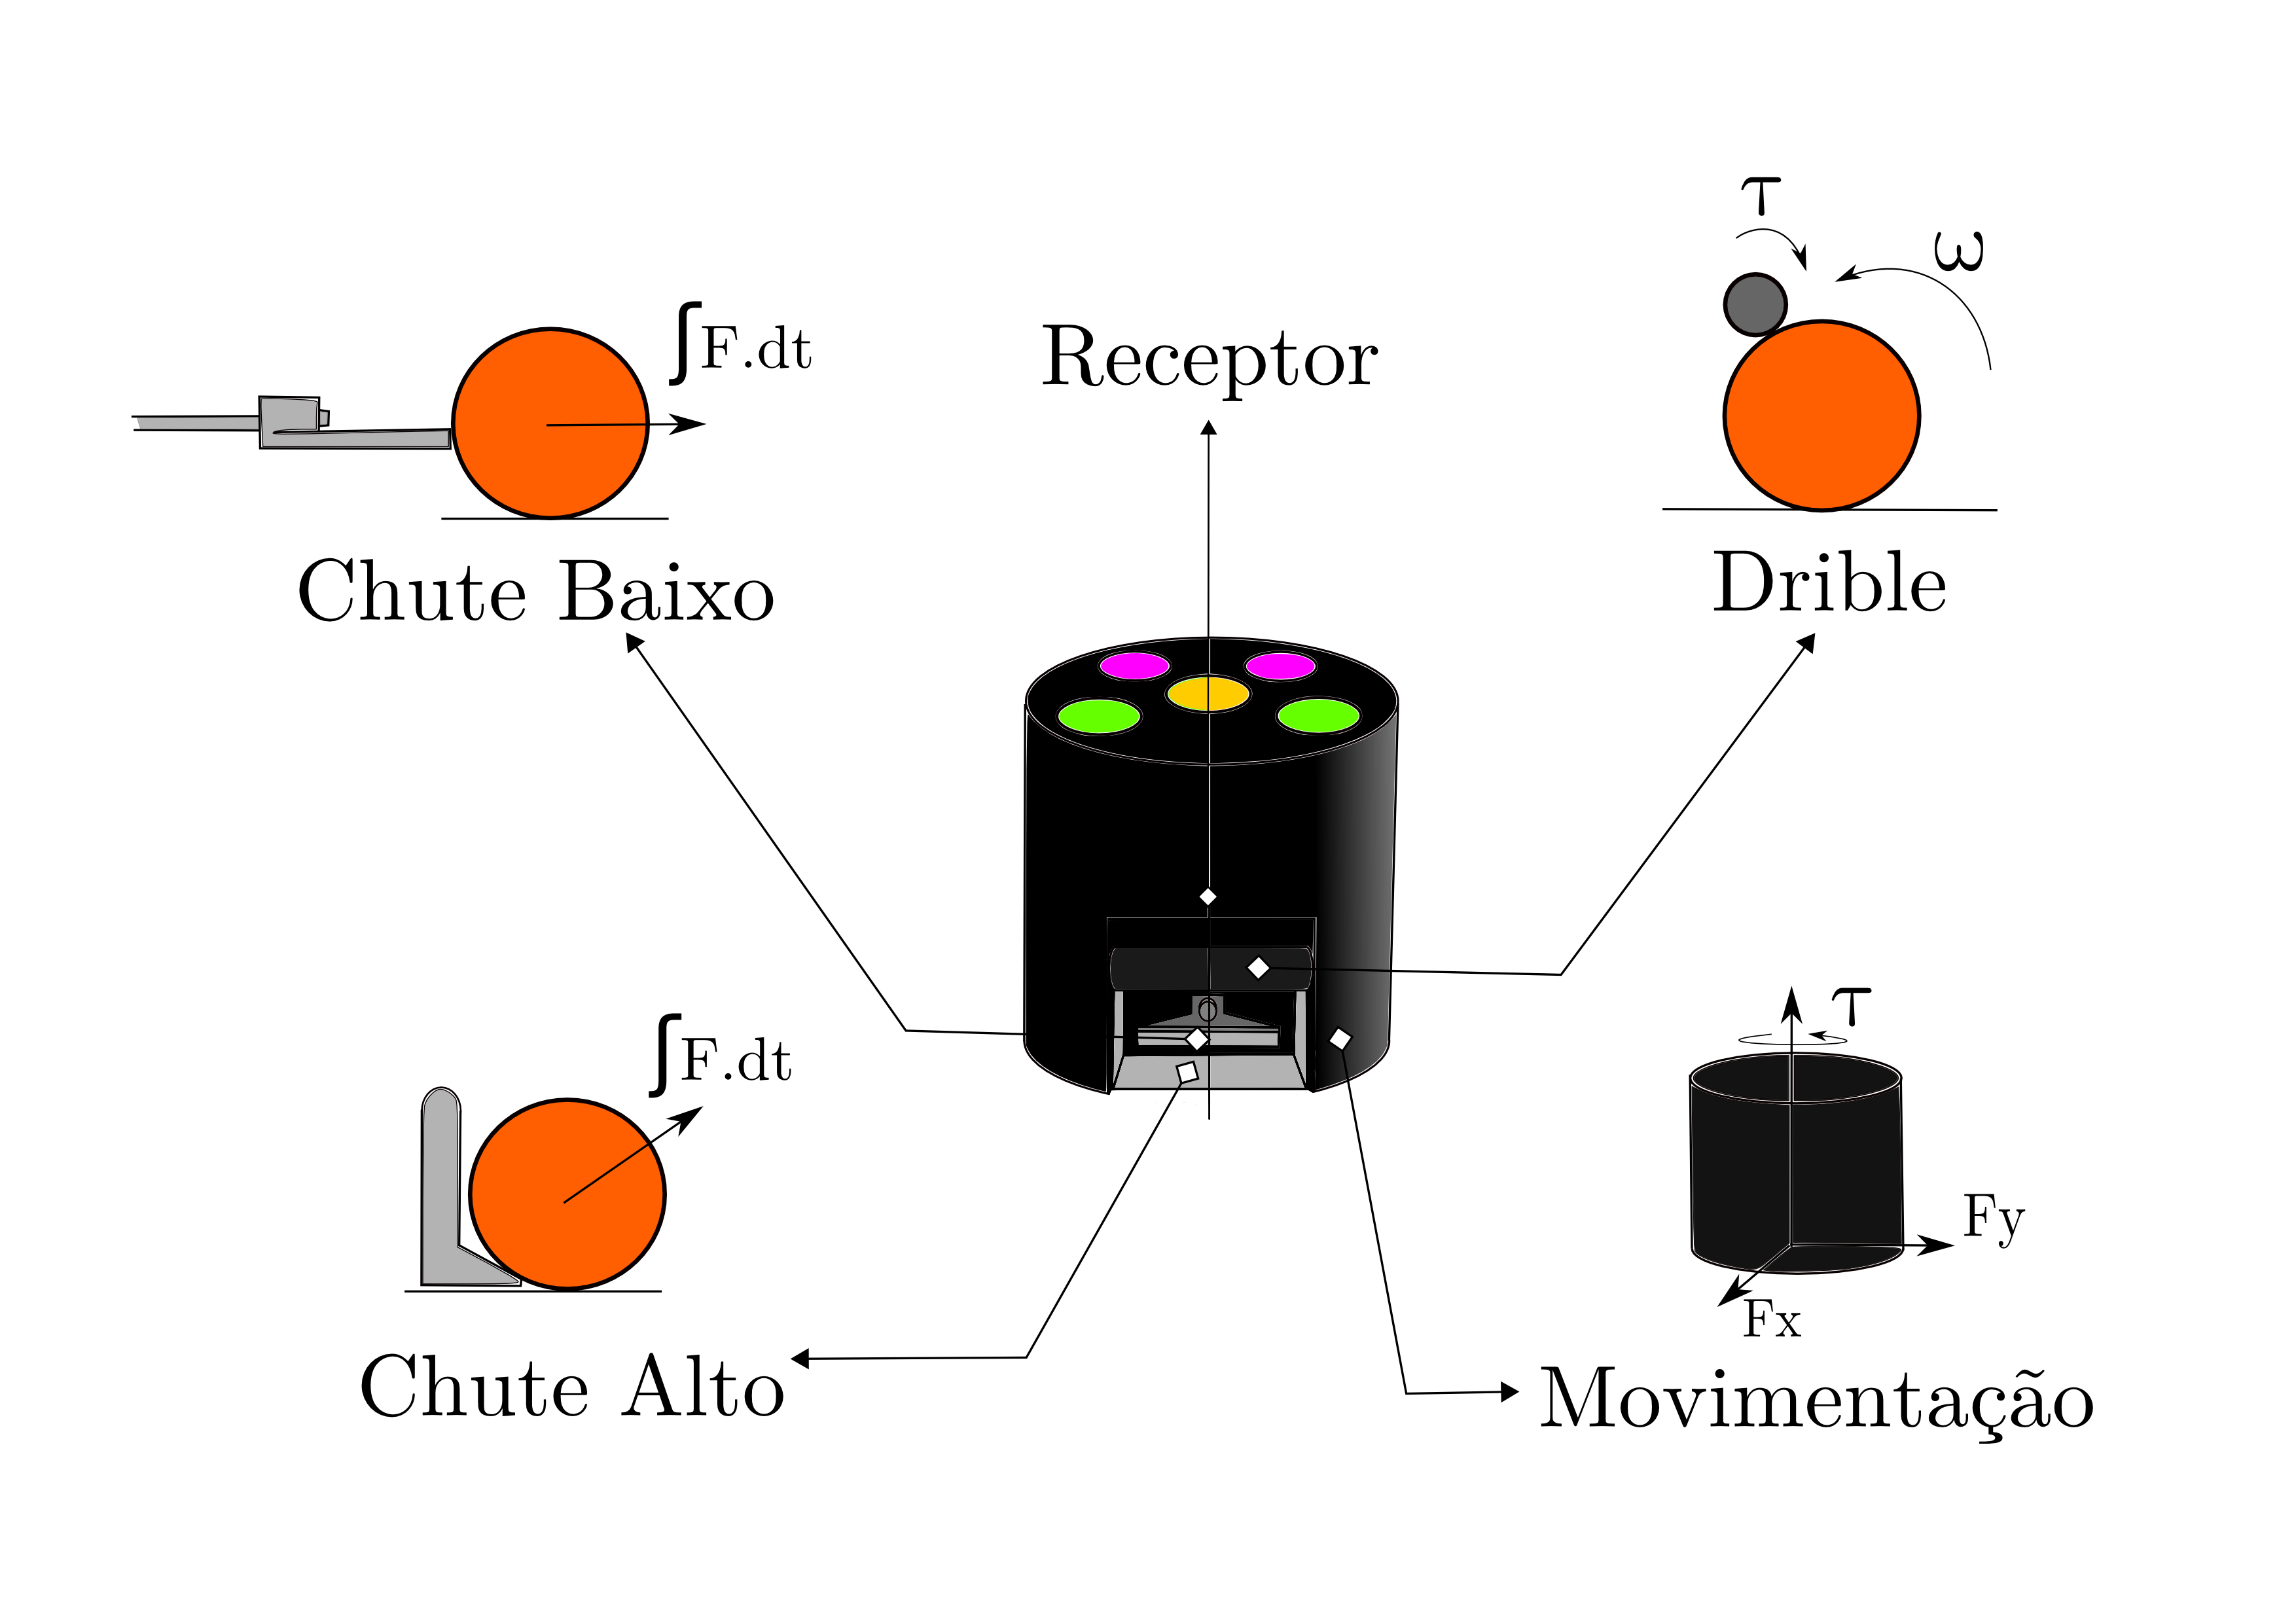
\includegraphics[width=0.8\linewidth]{robo}
    \caption{Atuadores típicos de um robo da SSL}\label{fig:robo}
  \end{figure}

  Apesar de o modelo descrito acima abranger a maioria dos
  robôs utilizados atualmente por equipes da SSL, é importante
  ressaltar que o robô pode ter um conjunto de sensores que
  poderiam coletar informações adicionais às transmitidas pela
  \textit{SSL-Vision} juntamente com um sistema de transmissão
  para enviá-las ao software do seu respectivo time. Isso é
  interessante, pois, conforme observado na Definição~\ref{def:bola},
  o parâmetro $\hat{b}.\theta$ não é observável. Como o sistema de
  drible impõe um torque à bola, por meio de um sensor, é possível
  estimar o valor de $\hat{b}.\omega$. Sem esse sensor, não é possível
  prever com exatidão a trajetória da bola somente com informações de
  simulação ou da visão.


% TODO: referenciar zicler para exemplos de skills
% TODO: Discrever Skill
%\begin{defi}[Skill]
%  $Sk \subset A_{rob}$ um conjunto de \textit{skills};
%\end{defi}
%
%% TODO: Discrever Tactic
%\begin{defi}[Tactic]
%  $tk = G(V \in Sk, E \in {prob} )$ o conjunto de todas as táticas possíveis
%  formadas a partir de grafos orientados, em que os vértices são \textit{skills} $sk \in Sk$
%  e as arestas são $prob$ associadas a possibilidade de ocorrerem as transições
%  entre uma skill e outra;
%
%% XXX: wtf???
%  $prob: X \longrightarrow [0,1]$ uma distribuição de probabilidade, cujo argumento é
%  $x \in X$;
%\end{defi}
%
%% TODO: Definir agente baseado em utilidade
%\begin{defi}[Tactic]
%  $f_{U}: X \longrightarrow \mathbb{R^{+}} \cup\lbrace 0\rbrace$ uma função utilidade tal que
%  $f_{U}(x)$ reflate a utilidade do estado $x \in X$ um entre estados do mundo dado os estados;
%\end{defi}
%
%% TODO: Definir árvore de busca
%\begin{defi}[Árvore de Busca]
%  $AB =\lbrace V \subset X, E \subset A\rbrace$ uma árvore de busca;
%\end{defi}
%
%% TODO: Definir estratégia (pode ser o BK-BGK)
%\begin{defi}[Estratégia de Busca]
%  $e_b: \langle X_{ob}^{i}, e, f_{U}, r_i, AB\rangle \longrightarrow AB^{'}$ uma estratégia de busca.
%\end{defi}
%
%% TODO: Modelo de reação dos robôs do time adversário
%\begin{defi}[Modelo de reação dos robôs do time]
%  Depende de quão distante no tempo está a reação que se quer
%  estimar. Quanto menor a distância no tempo, mais este modelo
%  se aproxima do modelo dinâmico dos robôs.
%\end{defi}

\begin{defi}[Time]\label{def:time}
  Sejam os seguintes parâmetros:

  \begin{description}
    \item $Rob_c$ o conjunto dos robôs controlados;
    \item $Rob_{ad}$ o conjunto dos robôs adversários, isto é, não controlados;
    \item $X$ o espaço de estado de todos os corpos rígidos envolvidos na partida considerada;
    \item $x_{init} \in X$ o estado inicial;
    \item $X_{goal}\subset X$ o conjunto de estados objetivo;
    \item $x_{ob}^{i}$ os estados observados pelo módulo \textit{SSL-Vision} no instante $i$;
    \item $X_{ob}^{i} =  \lbrace{x_{ob}^{0} = x_{init},\dots,x_{ob}^{i}}\rbrace$;
    \item $Sk \subset A_{rob}$ um conjunto de \textit{skills};
    \item $prob: X \longrightarrow [0,1]$ uma distribuição de probabilidade, cujo argumento é
          $x \in X$;
    \item $tk = G(V \in Sk, E \in {prob} )$ o conjunto de todas as táticas possíveis
          formadas a partir de grafos orientados, em que os vértices são \textit{skills} $sk \in Sk$
          e as arestas são $prob$ associadas a possibilidade de ocorrerem as transições
          entre uma skill e outra;
    \item $A_c = A_{rob 1} \cup \dots \cup A_{rob n_c}$ o conjunto das ações possíveis de $Rob_c$;
    \item $A_{ad} = A_{rob 1} \cup \dots \cup A_{rob n_{ad}}$ o conjunto das ações possíveis de $Rob_{ad}$;
    \item $A = A_c \cup A_{ad}$ o conjunto das ações possíveis de $Rob_c \cup Rob_{ad}$;
    \item $e: \langle x,a \rangle \longrightarrow x^{'}$ a função de transição de estado que pode
          aplicar uma ação $a\in A$ em um estado particular
          $x \in X$ e computar o estado seguinte $x^{'} \in X$;
    \item $f_{U}: X \longrightarrow \mathbb{R^{+}} \cup\lbrace 0\rbrace$ uma função utilidade tal que
          $f_{U}(x)$ mede a utilidade do estado $x \in X$ um entre estados do mundo dado os estados;
    \item $m_{reac{\ }ad}: \langle A_{ad}, X_{ob}^{i}\rangle \longrightarrow a_{ad}^{'}$ o modelo de reação dos robôs
          adversários dado $X_{ob}^{i}$;
    \item $AB =\lbrace V \subset X, E \subset A\rbrace$ uma árvore de busca;
    \item $e_b: \langle X_{ob}^{i}, e, f_{U}, m_{reac{\ }ad}, AB\rangle \longrightarrow AB^{'}$ uma estratégia de busca.
  \end{description}

  Então, um time $T$ é definido por:
  \[
    T: \langle Rob_c, A, X_{ob}^{i}, e, e_b, m_{reac{\ }ad} \rangle \longrightarrow a_c^{i+1}
  \]
\end{defi}

  Assim, utilizando-se de $e$, $T$ pode simular várias sequência de ações $a_c$ dado $X_{ob}^{i}$
  a partir de $f_{U}$ e $e_b$. Pode-se, a partir de $m_{reac{\ }ad}$, considerar as ações do time
  adversário baseado em estados anteriores.

% TODO: describe more the notation
\begin{defi}[Partida]
  Dado dois times $T_1$ e $T_2$. Uma partida $p$ é definida por:

  \[
   p = \lbrace T_1, T_2, \Delta t, \delta t, \langle Ref^{0}, X_{ob}^{0}, A_1^{0}, A_2^{0}\rangle, 
    \dots, \langle Ref^{N}, X_{ob}^{N}, A_1^{N}, A_2^{N} \rangle \rbrace
 \]

  uma sequência , em que:
  \begin{description}
    \item $\Delta t$ é o tempo de duração da partida;
    \item $\delta t$ é o tempo médio entre cada frame enviado pela \textit{SSL-Vision} ao longo de $\Delta t$;
    \item $N \approxeq \frac{\Delta t}{\delta t}$ é número total de frames enviados pela \textit{SSL-Vision}
  ao longo de $\Delta t$;
    \item $Ref^{i}$ são os comandos enviados pelo módulo \textit{Referee-Box} no instante $i$;
    \item $X_{ob}^{i}$ são os dados enviados pelo módulo \textit{SSL-Vision} no instante $i$;
    \item $A_1^{i}$ são as ações executadas por $T_1$ no instante $i$;
    \item $A_2^{i}$ são as ações executadas por $T_2$ no instante $i$.
  \end{description}
\end{defi}

  Conforme citado em na Seção~\ref{sec:arch_ssl}, $\delta t$ normalmente é $16,6{\ }ms$.
  Um exemplo de $A^{i}$ pode ser visto na Figura~\ref{fig:default_atq}.

\begin{defi}[Logs]
  Dada uma partida $p$. O $log$ de $p$ é definidor por:

  \[
    log(p) = \lbrace p.\langle Ref^{0}, X_{ob}^{0}\rangle, \dots, p.\langle Ref^{N}, X_{ob}^{N}\rangle \rbrace
  \]
\end{defi}
 
  A principal diferença entre uma partida $p$ e $log$ é o desconhecimento das ações que levaram
  aos movimentos observados nas partidas. Isso é um metadado importante quando se quer utilizar
  os dados de um jogo para aproximar o comportamento de algum time (i.e., $m_{reac{\ }ad}$).
  Este é um problema que está fora do escopo deste trabalho. Um exemplo de uma abordagem para
  esse problema pode ser encotrado em \cite{vail2008crf}.

% vim: tw=80 et ts=2 sw=2 sts=2 ft=tex


\subsection{}

\section{Função Objetivo}
A função objetivo $f_U$ é definida pela seguinte
expressão:

\begin{dmath}
  f_U = \sum c_i 
\end{dmath}

Onde $\lbrace c_i \rbrace$ é o conjunto formado por custos. Os pesos de
cada custo serão denotados por $p_{descrição}$. São eles:
% TODO: Eu tirei a penalização, mas talvez seja melhor explicar
\begin{enumerate}
  \item Custo da Abertura do Gol
  \item Correção da Abertura do Gol Devido a Movimentação da Bola
  \item Distância Total das Ações $Mover(r)$
  \item Distância Máxima das Ações $Mover(r)$
  \item Mudança do Planejamento da Move Table
  \item Custo do Ataque
  \item Custo das Aberturas vistas por $r \in T_c$
  \item Custo das Aberturas vistas por $r \in T_{ad}$
  \item Custo da Defesa
  \item Número de Receptores
  \item Penalização por Próximidade do Gol do Adversário
  \item Penalização por Proximidade
\end{enumerate}

Além dos parâmetros listados acima, outros parâmetros
afetam o comportamento do time:
\begin{enumerate}
  \item Abertura do gol mínima para chute à gol
  \item Número de ramificações
\end{enumerate}

Esses parâmetros foram os primeiros utilizados no programa.
Ao longo dos testes realizados, foram criados novos parâmetros.
Entretanto, os parâmetros listados são suficientes para ilustrar
a mudança no comportamento do time.

% OBS: o Maj Duarte circulou o título, mas não sei se foi
%      pelos dois erros de português que tinha aqui...
\subsection{Custo da Abertura do Gol}\label{subsec:custo_gap}
O objetivo deste parâmetro é valorizar as aberturas maiores
de acordo com a soma total das aberturas com relação a cada
$r \in T$ e com aberturas maiores.
O cálculo deste custo é feito da seguinte maneira:

\begin{multline} 
 c_{abertura{\ }gol} = taxa_{abertura{\ }total/max{\ }gol} .
   \sum_{r_i \in T} abertura{\ }gol(bola, r)\\
   + (1 - taxa_{abertura{\ }total/max{\ }gol}) .
   max \lbrace abertura{\ }gol(bola, r): r \in T \rbrace 
\end{multline}

As aberturas são calculadas de acordo com a posição de um determinado robô $r$ (obstáculo)
e a posição atual da bola. Isso gera um conjunto de segmentos de reta
$\lbrace abertura{\ }gol(bola, r): r \in T \rbrace$.

Este custo afeta diretamente os seguintes custos:
\begin{itemize}
  \item Custo do Ataque
  \item Custo da Defesa
  \item Custo das aberturas do gol vistas por $r\in T_c$
  \item Custo das aberturas do gol vistas por $r\in T_{ad}$
\end{itemize}

\subsection{Correção da Abertura do Gol Devido a Movimentação da Bola} 
O objetivo deste parâmetro é incorporar a movimentação
da bola pelo atacante no cálculo da abertura do gol. Isso é importante,
pois defensores mais
próximos são mais facilmente driblados que defensores mais distantes. Isso
pode ser visualizado na figura \ref{fig:kick_pos}, onde foi considerada
uma variação de 15cm e de 0cm. Essa variação é medida na linha normal
à reta formada pela bola e pelo robô em questão.

% TODO: Adicionar gráfico detalhado as contas
%       vide arquivo board.cpp para detalhes de implementação

\begin{figure}[H]
  \centering
  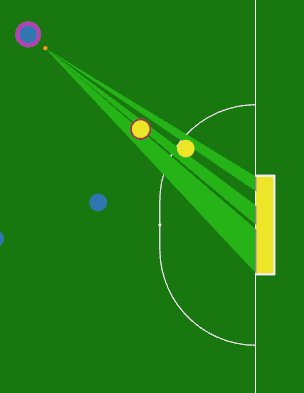
\includegraphics[height=0.4\linewidth]{kick_pos_var_1}
  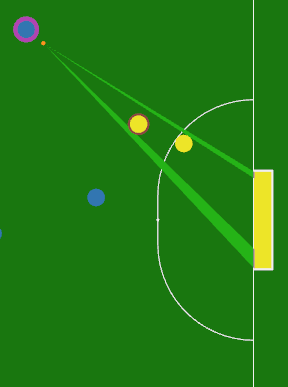
\includegraphics[height=0.4\linewidth]{kick_pos_var_2}
  \caption{Abertura do gol considerando-se uma variação de 15cm na 
           posição da bola (esquerda) e sem variação (direita)}\label{fig:kick_pos}
\end{figure}


\subsection{Distância Total das Ações $Mover(r)$} 
O objetivo deste parâmetro é valorizar o custo da
mudança de estado na função objetivo. Ele é formado pela soma das
distâncias que cada ação $Mover(r)$ irá percorrer partindo das
respectivas posições do estado atual.

\begin{dmath} 
 c_{dist{\ }total{\ }mover} = p_{dist{\ }total{\ }mover} . 
 \sum_{r_i \in T_c} \lVert pos_{r_i} - Mover(r_i)\rVert
\end{dmath} 

\subsection{Distância Máxima das Ações $Mover(r)$} 
O objetivo deste parâmetro é incorporar o custo da
mudança de estado na função objetivo. Ele é formado pela
ação $Mover(r)$ do planejamento atual com maior deslocamento.

\begin{gather} 
 c_{dist{\ }max{\ }mover}= p_{dist{\ }max{\ }mover} . 
 max \lbrace r_i \in T_c : \lVert pos_{r_i} - Mover(r_i)\rVert \rbrace
\end{gather} 

\subsection{Mudança do Planejamento da Tabela de Decisão}\label{subsec:change_cost}
O objetivo deste parâmetro é evitar mudanças grandes no
planejamento da ação $Mover(r)$. Uma das razões para isso é evitar um modelo dinâmico
exato neste nível de planejamento, já que isso aumentaria muito o custo
computacional desta etapa do planejamento e, consequentemente, reduziria
o número de simulações possíveis. Por essas razões mudanças no planejamento
das ações $Mover(r)$ inicialmente foram penalizadas de acordo com a distância euclidiana
entre o $Mover_p(r)$ planejado anteriormente e o $Mover_{m}(r)$ modificado, conforme
a equação:

\begin{dmath} 
 c_{mudança{\ }mover} = p_{mudança{\ }mover} . 
 max \lbrace \sum_{r_i \in T_c} \lVert Mover(r_i) - Mover_p(r_i)\rVert \rbrace
\end{dmath} 

Isso permite que sejam selecionados $Mover_{m}(r)$ mais próximos do
$Mover_p(r)$, refinado assim o planejamento anterior. Entretanto,
um parâmetro mais significativo é o valor absoluto do ângulo entre
essas ações e a posição de $r$, $\lVert ang(r, Mover_{m}(r), Mover_p(r)) \rVert$.
Dessa maneira, tem-se que este custo é computado da seguinte maneira:

\begin{dmath} 
 c_{mudança{\ }mover} = p_{mudança{\ }mover} . 
 max \lbrace \sum_{r_i \in T_c} \lVert ang(r, Mover_{m}(r), Mover_p(r)) \rVert \rbrace
\end{dmath} 

\subsection{Custo do Ataque}
Este custo valoriza situações nas quais o time em questão
possue o domínio da bola (descrito na Subsecção~\ref{subsec:repres_jogo}).

\begin{dmath} 
 c_{ataque} = p_{ataque} . abertura{\ }gol_{ad}
\end{dmath} 

Onde $abertura{\ }gol_{ad}$ é o valor da abertura do gol adversário visto
pelo robô que tem domínio da bola.

\subsection{Custo da Defesa}
Quando não se tem o domínio da bola a abertura do gol do time em questão
visto pelo robô do time adversário que tem a bola é utilizado
como penalização adicional.

\begin{dmath}
  c_{defesa} = p_{defesa} .
   \sum_{r_i \in T_ad} abertura{\ }gol_c(r_i)
\end{dmath}

\subsection{Custo das Aberturas do Gol Vistas por $r\in T_c$}

Este custo tem o objetivo de valorizar configurações nas quais
os robôs que não tem a bola possuam visada para o gol do time
adversário. Isso
é desejavel, já que permite que um gol seja feito caso o robô
que esta com a posse de bola execute um passe para um dos robôs
em questão.

\begin{dmath}
   c_{abertura{\ }gol{\ }ad} = p_{abertura{\ }gol_{ad}} .
    \sum_{r_i \in T_c} abertura{\ }gol_{ad}(r_i)
\end{dmath}

\subsection{Custo das Aberturas do Gol Vistas por $r\in T_{ad}$}

Este custo é o análogo do custo anterior, mas para o
time adversário. Ele visa penalizar situações nas quais
os robôs adversários tenham grande visada (i.e., abertura)
para o gol. 

\begin{dmath}
   c_{bloqueio{\ }gol} = - p_{bloqueio{\ }gol} .
    \sum_{r_i \in T_{ad}} abertura{\ }gol_{ad}(r_i)
\end{dmath}

\subsection{Número de Receptores}

Este custo visa valorizar cituaçõe nas quais existam
vários robôs que possam receber passe.

\begin{dmath}
  c_{receptores} = p_{receptores} .
   num \lbrace r_{receptor_i} \rbrace
\end{dmath}

\subsection{Penalização por Próximidade do Gol do Adversário}
Esta penalização visa evitar que os robôs que estão no ataque
se concentrem dentro da área do time adversário. Caso este
parâmetro não seja adicionado, é esse o comportamento resultante
do custo das aberturas vistas pelos robôs do time em questão. 
A partir de uma determinada distância, é adicionada uma parcela
de penalização na função objetivo.

\begin{dmath}
  c_{penalização{\ }prox} = - p_{penalização{\ }prox}
    \sum num \lbrace r_{perto} \rbrace
\end{dmath}

\subsection{Abertura Mínima para Chute a Gol}
Este parâmetro é o ângulo total da abertura do gol para permitir
o chute pelo atacante. Ele é relevante, pois afeta o comportamento
do atacante e, como consequência, o comportamento do time durante
a posse de bola. Quando a abertura do gol é menor que este valor, o
atacante tem ação de chutar em direção ao goal.

% TODO: Adicionar imagem para ilustrar este caso, já que não tem
%       equações envolvidas

\subsection{Número da Ramificação}
Este parâmetro é o número de possibilidades que serão simulados
em cada iteração do algorítmo de avaliação. Ele influencia o
tempo de resposta do planejamento.


\chapter{Arquitetura do Sistema}\label{cap:arquitetura}

Este capítulo descreve como a ferramenta desenvolvida interage com os
\textit{softwares} em uso na competição.

Os seguintes \textit{softwares} externos são de relevância para o entendimento
da arquitetura escolhida:

\begin{itemize}
  \item ssl-vision: desenvolvido pela comunidade e de uso oficial na competição
    para processamento das imagens da câmera nas partidas e distribuição pela
    rede dos dados processados (estado do jogo);
  \item grSim: desenvolvido pela comunidade e amplamente usado pelas equipes
    para simular o ambiente das partidas, o protocolo usado para enviar o estado
    pela rede é identico ao do ssl-vision;
  \item pyroboime: também chamado de core desenvolvido pela RoboIME, atualmente
    provê uma camada de abstração sobre a comunicação com o ambiente de jogo
    (real ou simulado) incluindo redução de ruído, planejamento de trajetória e
    controle.
\end{itemize}

Para fins práticos o desenvolvimento ocorre com validações no simulador (grSim).
O comportamento é compatível com as partidas oficiais.

\section{Comunicação com Componentes Externos}

\begin{figure}[H]
  \centering
  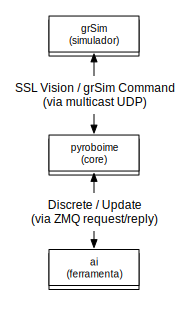
\includegraphics[height=10cm]{communication}
  \caption{Diagrama de comunicação entre os componentes.}\label{fig:arch-comm}
\end{figure}

A figura~\ref{fig:arch-comm} representa como os componentes se comunicam.  A
ferramenta se comunica apenas com o pyroboime para aproveitar todas as
funcionalidades necessárias que fogem ao escopo desse trabalho.  Por isso o foco
do desenvolvimento está concentrado em atender diretamente os objetivos.

As mensagens trocadas entre a ferramenta e o core (\textit{pyroboime}) é
codificada com o \textit{Protobuf}, uma biblioteca bem estabelecida que também é
usada nos protocolos oficiais da competição.  Desse modo o \textit{overhead} de
comunicação é baixo, não é necessário introduzir uma dependência ou codificação
manual no core e é possível que versões futuras sejam retrocompatíveis.

São dois tipos de mensagens:

\begin{itemize}
  \item atualização do estado: sentido do core para a ferramenta, codificadas
    com a mensagem UpdateMessage, descreve todas as informações necessárias para
    criar um estado novo;
  \item comando de ações: sentido ferramenta para o core, codificadas com a
    mensagem CommandMessage, descreve a ação que cada agente (robô) deve
    realizar.
\end{itemize}

As especificações de ambas as mensagens se encontram no anexo~\ref{att:protos}.

As mensagens são transmitidas num socket ZMQ (\textit{ZeroMQ}, uma biblioteca de
transmissão de dados na rede) visando a extensibilidade da ferramenta, pois com
tal biblioteca é possível distribuir mensagens entre vários nós de forma
confiável (característica desejável para um sistema distribuido) além de provêr
confiabilidade e auto-reconexão para o uso atual.

O modo de transmissão é \textit{request-reply} em que a ferramente age como
servidor respondendo as requisições do core, que consistem em atualizações cuja
a resposta deve ser o comando a ser executado naquele estado requisitado.  Na
prática a ferramenta irá transmitir o comando mais recente, que se encontra em
seu \textit{buffer}, descrito brevemente no seção~\ref{sec:threads}.

\section{\textit{Threads} do Sistema}\label{sec:threads}

\begin{figure}[H]
  \centering
  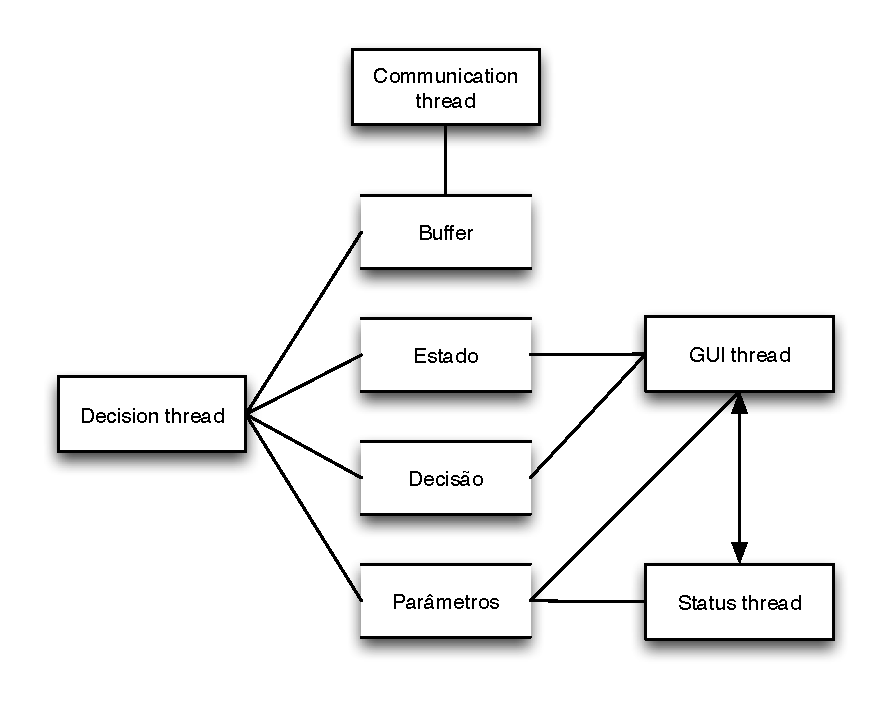
\includegraphics[height=10cm]{threads}
  \caption{Diagrama de relação entre \textit{threads} e
  dados.}\label{fig:arch-threads}
\end{figure}

A ferramenta está implementada em 4 \textit{threads} fixas de acordo com a
figura~\ref{fig:arch-threads}.  A separação foi motivada por:

\begin{itemize}
  \item A interface gráfica necessitar ser responsiva ao usuário;
  \item A taxa de tomada de decisão poder ser mais lenta que a taxa de
    atualização do estado, portanto a comunicação tem sua própria
    \textit{thread} que escreve e lê de um buffer compartilhado pela
    \textit{thread} de tomada de decisão;
  \item Certas informações devem ser coletadas periódicamente para atualizar
    alguns parâmetros e exibidas para o usuário.
\end{itemize}

\section{API Pública}

% TODO: um diagrama de colaboração de classes seria útil aqui

Uma API consiste nas estruturas e funções (ou também métodos) que estão
disponíveis para o programador.  A ferramenta está programada de forma que
também é possível fazer o uso programático de suas funcionalidades.

Esta seção descreve com detalhes cada estrutura e função presente na API da
ferramenta.  É um objetivo desta seção documentar o código da ferramenta para
possibilitar a evolução dessa em projetos futuros ou integração em outros
projetos.

Todas as estruturas e funções estão expostas em \textit{headers} C++, porém esta
documentação irá tratar apenas das funcionalidades e organização sem prender à
sintaxe ou modo de uso na linguagem em que está programada.  Para tais detalhes
o anexo~\ref{att:headers} pode ser consultado, esse contém o conteúdo dos
headers tratados nesta seção.

\subsection*{Enumeração \textit{ActionType}}

Representa o tipo da ação.

\subsubsection*{Alternativas}

\begin{itemize}
  \item \textit{NONE}: nenhuma ação;
  \item \textit{MOVE}: acão de movimentação;
  \item \textit{PASS}: ação de passe;
  \item \textit{KICK}: ação de chute.
\end{itemize}

\subsection*{Estrutura \textit{Action}}

Representa a ação individual a ser executada por um robô, não está amarrada à um
robô, essa associação deve ser feita pelo usuário da estrutura, isso permite uma
associação implicita baseada na ordem do vetor ou outros tipos de otimizações,
por esse motivo algumas funções recebem um Id de robô para saber qual robô usar
em certas circunstâncias.

\subsubsection*{Atributos}

\begin{itemize}
  \item \textit{type}: tipo (\textit{ActionType}), por padrão é do tipo NONE;
  \item \textit{move_pos}: posição destino da movimentação;
  \item \textit{kick_pos}: posição alvo do chute;
  \item \textit{pass_receiver}: Id do robô que deve receber o passe.
\end{itemize}

\subsubsection*{Métodos}

\begin{itemize}
  \item \textit{make_move_action}
    \par Entrada: vetor indicando um destino.
    \par Saída: ação do tipo MOVE.
  \item \textit{make_kick_action}
    \par Entrada: vetor indicando um alvo.
    \par Saída: ação do tipo KICK.
  \item \textit{make_pass_action}
    \par Entrada: Id de robô, que irá receber o passe.
    \par Saída: ação do tipo PASS.
  \item \textit{gen_move_action}
    \par Entrada: Id de um robô, estado, tabela de decisão.
    \par Saída: ação do tipo MOVE aleatória, que não colide com a posição de
    nenhum outro robô, nem com a posição destino desses de acordo com a tabela
    de decisão.
  \item \textit{gen_kick_action}
    \par Entrada: Id de um robô, estado, tabela de decisão.
    \par Saída: ação do tipo KICK no ponto de maior abertura do gol do inimigo
    que continuar aberto após as movimentações da tabela de decisão.  É assumido
    que um chute é possível e isso foi verificado previamente.
  \item \textit{gen_pass_action}
    \par Entrada: Id de um robô, estado, tabela de decisão.
    \par Saída: ação do tipo PASS aleatória para algum robô (do mesmo time) que
    possa receber o passe, o critério para receber o passe envolve que o
    receptor chegue em seu destino antes que o passador consiga chegar na bola e
    chuta-lá até o destino do receptor, além disso após o chute o receptor deve
    conseguir ser o dono da bola.
  \item \textit{gen_primary_action}
    \par Entrada: Id de um robô, estado, tabela de decisão, flag que indica se é
    de chute.
    \par Saída: ação do tipo KICK ou PASS, simplesmente abstrai
    \textit{gen_pass_action} ou \textit{gen_kick_action} para evitar verbosidade.
  \item \textit{apply_to_state}
    \par Entrada: ação, Id do robô, referência para um estado.
    \par Efeito: aplica a ação a um estado.  É assumido que a ação pode ser
    aplicada.  Ações de chute levam a bola para o gol.
\end{itemize}

%#ifndef CONSTS_H
%#define CONSTS_H
%
%constexpr int N_ROBOTS = 6;
%constexpr int MAX_SUGGESTIONS = 30;
%constexpr int MAX_SUGGESTION_SPOTS = 30;
%
%// Units are SI: m, m/s, s, ...
%
%constexpr float LINE_WIDTH = 0.010;
%constexpr float FIELD_WIDTH = 8.090;
%constexpr float FIELD_HEIGHT = 6.050;
%constexpr float GOAL_WIDTH = 1.000;
%constexpr float GOAL_DEPTH = 0.180;
%constexpr float GOAL_WALL_WIDTH = 0.020;
%constexpr float CENTER_CIRCLE_RADIUS = 0.500;
%constexpr float DEFENSE_RADIUS = 1.000;
%constexpr float DEFENSE_STRETCH = 0.500;
%constexpr float BOUNDARY_WIDTH = 0.500;
%constexpr float REFEREE_WIDTH = 0.250;
%constexpr float ROBOT_RADIUS = 0.180 / 2;
%constexpr float BALL_RADIUS = 0.043 / 2;
%constexpr float ROBOT_MAX_SPEED = 1.0;
%constexpr float ROBOT_KICK_SPEED = 6.0;
%constexpr float MAX_PASS_DISTANCE = 2.5;
%
%constexpr const char *PROGRAM_NAME =
%    "AI for RoboIME"; // TODO: better name maybe?
%constexpr int GUI_DEFAULT_WIDTH = 944;
%constexpr int GUI_DEFAULT_HEIGHT = 740;
%
%enum _ParamGroup {
%  MAX_ATTACK = 0,
%  MIN_ATTACK = 1,
%  MAX_CONQUER = 2,
%  MIN_CONQUER = 3
%};
%
%extern const int *const PARAM_GROUP;
%extern bool PARAM_GROUP_AUTOSELECT;
%extern bool PARAM_GROUP_CONQUER;
%extern float PARAM_GROUP_THRESHOLD;
%extern float PARAM_GROUP_CONQUER_TIME;
%void set_param_group(int new_param_group);
%
%#ifdef _CONST_IMPL
%#define PARAM(TYPE, NAME, DEFAULT) _CONST_IMPL(TYPE, NAME, DEFAULT)
%#else
%#define PARAM(TYPE, NAME, DEFAULT) extern TYPE NAME;
%#endif
%
%PARAM(bool, CONSTANT_RATE, true);
%PARAM(bool, KICK_IF_NO_PASS, false);
%PARAM(int, DECISION_RATE, 7);
%PARAM(int, RAMIFICATION_NUMBER, 5000);
%PARAM(int, FULL_CHANGE_PERCENTAGE, 100);
%PARAM(int, MAX_DEPTH, 0);
%PARAM(float, KICK_POS_VARIATION, 0.150);
%PARAM(float, MIN_GAP_TO_KICK, 18.0);
%PARAM(float, DESIRED_PASS_DIST, 2.0);
%PARAM(float, WEIGHT_BALL_POS, 0);
%PARAM(float, WEIGHT_MOVE_DIST_MAX, 0);
%PARAM(float, WEIGHT_MOVE_DIST_TOTAL, 0);
%PARAM(float, WEIGHT_MOVE_CHANGE, 2);
%PARAM(float, WEIGHT_PASS_CHANGE, 2);
%PARAM(float, WEIGHT_KICK_CHANGE, 2);
%PARAM(float, TOTAL_MAX_GAP_RATIO, 0.5);
%PARAM(float, WEIGHT_CLOSE_TO_BALL, 1000);
%PARAM(float, WEIGHT_ENEMY_CLOSE_TO_BALL, 1000);
%PARAM(float, WEIGHT_HAS_BALL, 5000);
%PARAM(float, WEIGHT_ATTACK, 1000);
%PARAM(float, WEIGHT_SEE_ENEMY_GOAL, 10);
%PARAM(float, WEIGHT_BLOCK_GOAL, 180);
%PARAM(float, WEIGHT_BLOCK_ATTACKER, 5000);
%PARAM(float, WEIGHT_GOOD_RECEIVERS, 0);
%PARAM(float, WEIGHT_RECEIVERS_NUM, 20);
%PARAM(float, WEIGHT_ENEMY_RECEIVERS_NUM, 20);
%PARAM(float, DIST_GOAL_PENAL, 2000);
%PARAM(float, DIST_GOAL_TO_PENAL, 1.0);
%PARAM(float, MOVE_RADIUS_0, 0.5);
%PARAM(float, MOVE_RADIUS_1, 2.0);
%PARAM(float, MOVE_RADIUS_2, 7.0);
%
%enum Weight {
%  _WEIGHT_BALL_POS,
%  _WEIGHT_MOVE_DIST_MAX,
%  _WEIGHT_MOVE_DIST_TOTAL,
%  _WEIGHT_MOVE_CHANGE,
%  _WEIGHT_PASS_CHANGE,
%  _WEIGHT_KICK_CHANGE,
%  _WEIGHT_CLOSE_TO_BALL,
%  _WEIGHT_ENEMY_CLOSE_TO_BALL,
%  _WEIGHT_HAS_BALL,
%  _WEIGHT_ATTACK,
%  _WEIGHT_SEE_ENEMY_GOAL,
%  _WEIGHT_BLOCK_GOAL,
%  _WEIGHT_BLOCK_ATTACKER,
%  _WEIGHT_GOOD_RECEIVERS,
%  _WEIGHT_RECEIVERS_NUM,
%  _WEIGHT_ENEMY_RECEIVERS_NUM,
%  _WEIGHT_PENALS,
%  W_SIZE
%};
%
%#ifndef _CONST_IMPL
%#undef PARAM
%#endif
%
%#endif

\subsection*{Estrutura \textit{Decision}}

Representa uma decisão total de um time, isto é todos os robôs irão possuir
ações, mesmo que sejam do tipo NONE.  Similarmente à uma ação individual, uma
decisão não está atrelada a um time, e por isso é comum alguns métodos
precisarem de uma decisão e o time a qual será aplicada.

\subsubsection*{Atributos}

\begin{itemize}
  \item \textit{action}: array de ações de tamanho igual ao número de robôs que
    um time possui.
\end{itemize}

\subsubsection*{Métodos}

\begin{itemize}
  \item \textit{apply_to_state}
    \par Entrada: decisão, time e referência a um estado.
    \par Efeito: todas as ações da decisão são aplicadas ao estado, assim como
    em uma ação é assumido que é possível aplicar a decisão.
  \item \textit{gen_decision}
    \par Entrada: flag que indica se é chute, estado, jogador, tabela de decisão
    e robô que irá se movimentar (opcional)
    \par Saída: decisão gerada aleatoriamente usando as restrições de geração de
    ações.  Caso um robô para se movimentar seja especificado esse será o único
    a receber uma movimentação aleatória os outros seguirão com as ações da
    tabela de decisão.
  \item \textit{to_proto_command}
    \par Entrada: decisão, time, referência para um mensagem
    \textit{CommandMessage}, tabela de Ids.
    \par Efeito: converte uma decisão para a estrutura de mensagem gerada pelo
    \textit{Protobuf}.
\end{itemize}

\subsection*{Enumeração \textit{DecisionSource}}

Representa de qual tipo de ramo uma decisão foi gerada.

\subsubsection*{Alternativas}

\begin{itemize}
  \item \textit{NO_SOURCE}: não há fonte, usado como padrão para decisões
    vazias.
  \item \textit{SUGGESTION}: decisão gerada a partir de uma sugestão (posição
    chave).
  \item \textit{TABLE}: decisão gerada a partir de uma tabela de decisão.
  \item \textit{FULL_RANDOM}: decisão gerada a partir de uma movimentação de
    todos os robôs.
  \item \textit{SINGLE_RANDOM}: decisão gerada a partir da movimentação de um
    único robô.
\end{itemize}

\subsection*{Estrutura \textit{DecisionTable}}

\subsubsection*{Atributos}

\begin{itemize}
  \item \textit{kick_robot}: Id do robô com ação de chute, é opcional, na
    ausência indica que não há robo com ação de chute.
  \item \textit{kick}: ação de chute.
  \item \textit{pass_robot}: Id do robô com ação de chute, é opcional, na
    ausência indica que não há robo com ação de chute.
  \item \textit{pass}: ação de passe.
  \item \textit{move}: array de ações de movimentação com tamanho igual ao
    número de robôs que um time possui.
\end{itemize}

%#ifndef DRAW_H
%#define DRAW_H
%
%#include "player.h"
%
%void screen_zoom(int width, int height, double zoom, double center_x,
%                 double center_y);
%void draw_state(const struct State &state);
%void draw_decision(const struct Decision &decision,
%                   const struct State &state, Player player);
%void draw_suggestion(const struct SuggestionTable &table);
%void draw_app_status(void);
%void draw_options_window(void);
%
%#endif

%#ifndef FILTER_H
%#define FILTER_H
%
%#include "array.h"
%
%// this is a exclusion filter, true means out
%// (rationale behind it is that default initialization goes to no
%// filter)
%struct TeamFilter : TeamArray<bool> {
%  int count = N_ROBOTS;
%};
%
%void filter_out(TeamFilter &team_filter, int i);
%
%#endif

\subsection*{Estrutura \textit{Optimization}}

Uma instância representa uma unidade de otimização.  A princípio seria
necessário apenas uma função otimizadora mas com existe persistência de
informações (como tabela de decisão) então foi criada essa estrutura para
persistir tais dados de maneira explícita.

\subsubsection*{Atributos}

\begin{itemize}
  \item \textit{table}: tabela de decisão.
  \item \textit{robot_to_move}: usado para fazer o rodízio do robô que irá ser
    movimentado no modo SINGLE_RANDOM.
  \item \textit{table_initialized}: flag para marcar se a tabela já foi
    inicializada, usado apenas para algumas otimizações.
\end{itemize}

\subsection*{Métodos}

\begin{itemize}
  \item \textit{decide}
    \par Entrada: instância de otimização, estado, time, sugestões (opcional)
    \par Saída: decisão valorada, número de ramificação (opcional)
\end{itemize}

\subsection*{Enumeração \textit{Player}}

Indica um time.

\subsubsection*{Alternativas}

\begin{itemize}
  \item \textit{MIN}: time cujo valor é minimizado, normalmente configurado como
    time inimigo.
  \item \textit{MAX}: time cujo valor é maximizado.
\end{itemize}

\subsection*{Estrutura \textit{Segment}}

Representa um segmento de uma dimensão, usado para cálculo de \textit{gaps}
(vãos) no gol.

\subsubsection*{Atributos}

\begin{itemize}
  \item \textit{u}: valor superior (up).
  \item \textit{d}: valor inferior (down).
\end{itemize}

\subsection*{Estrutura \textit{State}}

Representa o estado do jogo.  É importante ressaltar que os Ids usados dentro da
ferramenta têm significado diferente do Id usado no jogo.  Aqui os Ids são
únicos para cada robô, mesmo entre times, isto é, um Id usado pelo time MIN não
pode ser usado pelo time MAX.  Mais notável é que os Ids variam necessáriamente
entre $0$ e $11$ inclusive, sendo a primeira porção correspondente ao time MIN e
a segunda ao time MAX.  Esse design permite usar Ids como índices de arrays e
determinar o time a partir de um Id.  Para tanto é necessário uma tabela de Ids
para mapear para os Ids usados na partida.

\subsubsection*{Atributos}

\begin{itemize}
  \item \textit{ball}: vetor posição da bola.
  \item \textit{ball_v}: vetor velocidade da bola.
  \item \textit{robots}: array de vetores posição de cada robô do jogo.
  \item \textit{robots_v}: array de vetores velocidade de cada robô do jogo.
\end{itemize}

\subsection*{Métodos}

\begin{itemize}
  \item \textit{uniform_rand_state}
    \par Saída: estado uniformemente aleatório, usado apenas para testes.
  \item \textit{can_kick_directly}
    \par Entrada: estado, time.
    \par Saída: booleano, se o time é capaz de realizar um chute direto.
  \item \textit{robot_with_ball}
    \par Entrada: estado.
    \par Saída: Id do robô com a bola.
    \par Saídas opcionais: tempo para o time MIN alcançar a bola, tempo para o
    time MAX alcançar a bola, Id do robô do time MIN mais próximo à bola, Id do
    robô do time MAX mais próximo à bola.
    \par A posse de bola usa o tempo para chegar à bola, que leva em
    consideração a velocidade da bola.
  \item \textit{total_gap_len_from_pos}
    \par Entrada: estado, posição origem, time, robô a ser ignorado (opcional).
    \par Saída: soma de todas as aberturas vistas a partir da origem no gol do
    time especificado.
  \item \textit{max_gap_len_from_pos}
    \par Entrada: estado, posição origem, time, robô a ser ignorado (opcional).
    \par Saída: maior entre todas as aberturas vistas a partir da origem no gol do
    time especificado.
  \item \textit{time_to_pos}
    \par Entrada: vetor posição da origem, vetor velocidade da origem, vetor posição
    do destino, vetor velocidade do destino, velocidade máxima do ponto de
    origem (opcional, por padrão do robô).
    \par Saída: menor tempo para o ponto chegar da origem no destino assumindo
    aceleração infinita do ponto e velocidade constante do destino.
  \item \textit{discover_gaps_from_pos}
    \par Entrada: estado, posição de origem, jogador, robô a ser ignorado
    (opcional).
    \par Saída: array de segmentos e tamanho do array, contém todos os segmentos
    que representam os vãos (gaps) que podem ser observados no gol do time
    especificado.
  \item \textit{evaluate_with_decision}
    \par Entrada: time, estado, decisão, tabela de decisão.
    \par Saída: valor, valores individuais por peso (opcional)
    \par Essa é a função objetivo.
  \item \textit{discover_possible_receivers}
    \par Entrada: estado, tabela de decisão, jogador, Id do robô que faz o
    passe.
    \par Saída: lista dos robôs to time dado que podem receber passes.
  \item \textit{update_grom_proto}
    \par Entrada: referência para um estado, mensagem UpdateMessage, tabela de
    Ids.
    \par Efeito: atualiza o estado com os dados da mensagem se baseando no
    mapeamento da tabela de Ids.
\end{itemize}

\subsection*{Estrutura \textit{SuggestionTable}}

Tabela de sugestão, também referida por Posições Chaves.  Representa um conjunto
de posições chaves que é usado para gerar uma única decisão.

\subsubsection*{Atributos}

\begin{itemize}
  \item \textit{name}: nome do conjunto, útil para rótulos como 'barreira' ou
    '2-2-1' ou 'ataque pela direita'.
  \item \textit{spots_count}: contagem de posições.
  \item \textit{spots}: array de vetores posição.
  \item \textit{usage_count}: contagem de uso desta tabela, usado para
    estatísticas.
\end{itemize}

\subsubsection*{Métodos}

\begin{itemize}
  \item \textit{add_spot}
    \par Entrada: tabela de sugestão.
    \par Saída: novo tamanho da tabela, ou $-1$ em caso de erro.
    \par Efeito: adiciona uma posição na tabela.
  \item \textit{del_spot}
    \par Entrada: tabela de sugestão, posição a remover.
    \par Saída: novo tamanho da tabela, ou $-1$ em caso de erro.
  \item \textit{gen_decision}
    \par Entrada: flag indicando se decisão é de chute, tabela de sugestão,
    estado, tabela de decisão, time.
    \par Saída: decisão construída a partir da tabela de sugestão, o
    comportamento há menos posições que robôs é preencher com moves aleatórios e
    quando há mais posiçoes que robôs é usar as posições mais próximas há cada
    robô sem que haja repetição.
\end{itemize}

\subsection*{Estrutura \textit{Suggestions}}

Representa o conjunto de todas as tabelas de sugestões.

\subsubsection*{Atributos}

\begin{itemize}
  \item \textit{tables}: tabelas de sugestão.
  \item \textit{tables_count}: contagem de tabelas.
  \item \textit{last_use}: posição da última tabela usada para gerar uma decisão.
\end{itemize}

\subsubsection*{Métodos}

\begin{itemize}
  \item \textit{add_suggestion}
    \par Entrada: conjunto de sugestões.
    \par Saída: novo tamanho do conjunto, ou $-1$ em caso de erro.
    \par Efeito: adiciona uma posição no conjunto com uma tabela vazia.
  \item \textit{del_suggestion}
    \par Entrada: conjunto de sugestões, posição a remover.
    \par Saída: novo tamanho do conjunto, ou $-1$ em caso de erro.
  \item \textit{save_suggestions}
    \par Entrada: conjunto de sugestões, caminho de arquivo.
    \par Efeito: salva no arquivo o conjunto de sugestões em um formato textual.
  \item \textit{load_suggestions}
    \par Entrada: conjunto de sugestões, caminho de arquivo.
    \par Efeito: carrega do arquivo o conjunto de sugestões.
\end{itemize}

%#ifndef UTILS_H
%#define UTILS_H
%
%#include <cmath>
%
%#include "consts.h"
%#include "player.h"
%#include "vector.h"
%
%#define FOR_RANGE(I, F, T) for (int I = (F); I < (T); I++)
%#define FOR_N(I, N) FOR_RANGE(I, 0, N)
%#define FOR_N_IN(I, N, F) FOR_RANGE(I, 0, N) if (!F[I])
%#define FOR_EVERY_ROBOT(I) FOR_RANGE(I, 0, 2 * N_ROBOTS)
%#define FOR_TEAM_ROBOT(I, T)                                           \
%  FOR_RANGE(I, T *N_ROBOTS, (1 + T) * N_ROBOTS)
%#define FOR_EVERY_ROBOT_IN(I, F) FOR_EVERY_ROBOT(I) if (!F[I])
%#define FOR_TEAM_ROBOT_IN(I, T, F) FOR_TEAM_ROBOT(I, T) if (!F[I])
%
%constexpr int ROBOT_WITH_PLAYER(int R, Player P) {
%  return P * N_ROBOTS + R % N_ROBOTS;
%}
%
%constexpr Player ENEMY_FOR(Player P) { return P == MIN ? MAX : MIN; }
%constexpr Player PLAYER_OF(int R) {
%  return R / N_ROBOTS == MIN ? MIN : MAX;
%}
%constexpr Player ENEMY_OF(int R) { return ENEMY_FOR(PLAYER_OF(R)); }
%
%// 1 for MIN -1 for MAX
%constexpr int PLAYER_SIGN(Player P) { return P == MAX ? 1 : -1; }
%
%// XXX: MAX to the left, not taking into account that it may be
%// otherwise
%constexpr float GOAL_Y(Player) { return 0; }
%constexpr float GOAL_X(Player P) {
%  return -PLAYER_SIGN(P) * FIELD_WIDTH / 2;
%}
%constexpr Vector GOAL_POS(Player P) { return {GOAL_X(P), GOAL_Y(P)}; }
%
%// angle mesures conversions radians <-> degrees
%template <typename T> constexpr T RADIANS(T DEGREES) {
%  return M_PI * DEGREES / 180.;
%}
%template <typename T> constexpr T DEGREES(T RADIANS) {
%  return 180. * RADIANS / M_PI;
%}
%
%// a number squared
%template <typename T> constexpr T SQ(T X) { return X * X; }
%
%#endif

\subsection*{Estrutura \textit{ValuedDecision}}

Essa estrutura existe para anexar um valor à uma decisão, a intenção é que esse
seja um valor calculato pela função objetivo.  Uma alternativa seria usar tuplas
ou retornar o valor em um argumento de saída (pointeiro ou referência) mas a
estrutura é simples e possui uma semântica explícita e facilita evoluções, como
por exemplo a própria adição do attributo \textit{values}.

\subsubsection*{Atributos}

\begin{itemize}
  \item \textit{value}: valor associado à decisão.
  \item \textit{values}: array de valores que explicita quanto parcela da função
    objetivo contribui com o valor total, a soma dos valores será igual ao
    atributo \textit{value}.
  \item \textit{decision}: decisão associada ao valor.
\end{itemize}


\subsection*{Estrutura \textit{Vector}}

Vetor em duas dimensões usado para representar posições e velocidades no
programa.  Não deve ser confundido com um \textit{array}, que é uma sequência
de tamanho genérico (porém fixo) sem semântica associada.

\subsubsection*{Atributos}

\begin{itemize}
  \item \textit{x}: componente no eixo $x$.
  \item \textit{y}: componente no eixo $y$.
\end{itemize}

\subsubsection*{Métodos}

Alguns operadores foram definidos para essa estrutura de modo que suas operações
reflitam as operações matemáticas normalmente associadas a vetores.  Tais
operadores foram omitidos da lista de métodos mas podem ser consultados no
anexo~\ref{att:headers}.

\begin{itemize}
  \item \textit{norm2}
    \par Entrada: vetor.
    \par Saída: norma do vetor ao quadrado, usado para simplificar algumas
    operações, é ligeiramente menos custoso que a norma.
  \item \textit{norm}
    \par Entrada: vetor.
    \par Saída: norma do vetor.
  \item \textit{unit}
    \par Entrada: vetor.
    \par Saída: vetor com mesma direção porém norma unitária.
  \item \textit{uniform_rand_vector}
    \par Entrada: valor $r_x$, valor $r_y$.
    \par Saída: vetor aleatório distribuído uniformemente no região:
    $-r_x < x < r_x$, $-r_y < y < r_y$.
  \item \textit{normal_rand_vector}
    \par Entrada: vetor origem, valor sigma.
    \par Saída: vetor normalmente distribuído na origem e sigma entrados.
  \item \textit{rand_vector_bounded}
    \par Entrada: vetor origem, valor do raio, valores $r_x$ e $r_y$.
    \par Saída: vetor uniformemente distribuído em um círculo centrado na origem
    com o raio entrado que necessariamente está contido na região
    $-r_x < x < r_x$, $-r_y < y < r_y$, a segunda condição é sempre atendida nem
    que seja necessário quebrar a primeira.
  \item \textit{line_segment_cross_circle}
    \par Entrada: vetores $p_1$, $p_2$, vetor origem e valor do raio.
    \par Saída: verdadeiro se o segmento $(p_1, p_2)$ intercepta o círculo
    centrado na origem com o raio entrado.
  \item \textit{dist}
    \par Entrada: vetores $v_1$ e $v_2$.
    \par Saída: distância entre os vetores, sinônimo de $norm(v_1 - v_2)$.
\end{itemize}


% vim: tw=80 et ts=2 sw=2 sts=2 ft=tex

\chapter{Resultados}\label{cap:resultados}

\section{Influência dos Parâmetros no Comportamento do Time}
\subsection{Custo do gap}
\subsection{Correção do Gap devido a movimentação da bola}
\subsection{Distância Total dos Moves}
\subsection{Distância Máxima dos Moves} 
\subsection{Mudança do Planejamento da Move Table}
\subsection{Custo do Ataque}
\subsection{Custo dos gap vistos pelos robôs do time}
\subsection{Custo dos gaps vistos pelos robôs adversários}
\subsection{Custo da Defesa}
\subsection{Número de Receptores}
\subsection{Penalização por próximidade do gol do adversário}
\subsection{Penalização por proximidade}

\section{Interface Gráfica}


% ---
% Finaliza a parte no bookmark do PDF, para que se inicie o bookmark na raiz
% ---
\bookmarksetup{startatroot}%
% ---

%\addcontentsline{toc}{chapter}{Conclusão}
\chapter{Conclusão}\label{cap:conclusao}

% TODO:
% OBS: - Recontextualizar trabalho
%      - Retificação do cumprimento dos objetivos
%      - Listagem das contribuições
%      - Trabalhos futuros

Este trabalho objetiva desenvolver uma ferramenta de representação
comportamental baseada em otimização para futebol de robôs.  A meta
intermediária é criar um modelo discreto sequencial para o problema do futebol
de robôs. A partir desta discretização, foi desenvolvida uma arquitetura de
controle que seleciona jogadas o mais próximo da jogada ótima possível, de
acordo com uma função de avaliação e dentro do tempo disponível para o
planejamento.

Foi desenvolvido um modelo abstrato do futebol de robôs no
Capítulo~\ref{cap:modelagem}. Este modelo foi base para o programa apresentado
no Capítulo~\ref{cap:arquitetura}.

A ferramenta criada atingiu os objetivos desejados, modificando o comportamento
do time através da modificação dos parâmetros da função objetivo, conforme
mostrado no Capítulo~\ref{cap:resultados}. Também foi desenvolvida com sucesso
uma interface gráfica que permite modificar esses parâmetros em tempo de
execução.

O trabalho atual pode permitir que um time melhor seja criado modificando-se os
parâmetros da função objetivo ou adicionando novos custos à função objetivo.
Através do fornecimento dos parâmetros vencedores da competição anterior, tem-se
um avanço no desempenho do time.

Pode-se melhorar o time utilizando uma maneria automática para realizar as
partidas e avaliar o desempenho do time nessa partida. Isso permitiria que
algorítimos de otimização também fossem utilizados para melhorar os parâmetros.
Para isso, é a necessário um juíz automático para permitir jogos não
supervisionados por humanos.
% TODO: Escolher outra palavra, 'humanos' parece estranho.

% vim: tw=80 et ts=2 sw=2 sts=2 ft=tex


% ----------------------------------------------------------
% ELEMENTOS PÓS-TEXTUAIS
% ----------------------------------------------------------
\postextual


% ----------------------------------------------------------
% Referências bibliográficas
% ----------------------------------------------------------
%\bibliographystyle{plainnat}%abbrvnat, unsrtnat, apsrev, rmpaps, IEEEtranN, achemso, rsc
\bibliography{referencias}

% ----------------------------------------------------------
% Glossário
% ----------------------------------------------------------
%
% Consulte o manual da classe abntex2 para orientações sobre o glossário.
%
%\glossary

% ----------------------------------------------------------
% Apêndices
% ----------------------------------------------------------

% ---
% Inicia os apêndices
% ---
%\begin{apendicesenv}

% Imprime uma página indicando o início dos apêndices
%\partapendices

% ----------------------------------------------------------
%\chapter{Quisque libero justo}
% ----------------------------------------------------------
%\end{apendicesenv}
% ---


% ----------------------------------------------------------
% Anexos
% ----------------------------------------------------------

% ---
% Inicia os anexos
% ---
\begin{anexosenv}

% Imprime uma página indicando o início dos anexos
\partanexos

% ---
%\chapter{Morbi ultrices rutrum lorem.}
\chapter{Cabeçalhos}

\includecode{src/action.h}
%\includecode{adaptive_control.h}
\includecode{src/app.h}
\includecode{src/array.h}
%\includecode{src/colors.h}
\includecode{src/consts.h}
\includecode{src/decision.h}
\includecode{src/decision_source.h}
\includecode{src/decision_table.h}
\includecode{src/draw.h}
\includecode{src/filter.h}
%\includecode{src/gui.h}
\includecode{src/id_table.h}
\includecode{src/minimax.h}
\includecode{src/optimization.h}
\includecode{src/player.h}
\includecode{src/segment.h}
\includecode{src/state.h}
\includecode{src/suggestion_table.h}
\includecode{src/suggestions.h}
%\includecode{src/utils.h}
\includecode{src/valued_decision.h}
\includecode{src/vector.h}
\includecode{src/weight.h}

\chapter{Protocolos}

\includecode[proto]{proto/discrete.proto}
\includecode[proto]{proto/update.proto}

% vim: tw=80 et ts=2 sw=2 sts=2 ft=tex

% ---

\end{anexosenv}

%---------------------------------------------------------------------
% INDICE REMISSIVO
%---------------------------------------------------------------------

\printindex

\end{document}
% vim: tw=80 et ts=2 sw=2 sts=2 ft=tex
